\documentclass[compsoc,conference,a4paper,10pt]{IEEEtran}
% The preceding line is only needed to identify funding in the first footnote. If that is unneeded, please comment it out.
\pdfoutput=1
\usepackage{hyperref}       % hyperlinks
\usepackage{url}            % simple URL typesetting
\usepackage{booktabs}       % professional-quality tables
\usepackage{nicefrac}       % compact symbols for 1/2, etc.
\usepackage{microtype}      % microtypography
\usepackage{graphicx}
\usepackage{doi}
\usepackage{color}
\usepackage{xcolor}
\usepackage{cite}
\usepackage{colortbl}
\usepackage[font=footnotesize]{caption}
\usepackage{multicol}
\usepackage{amsmath,amsfonts,stmaryrd,xspace,enumitem}
\usepackage{tablefootnote}
\usepackage{multirow}
\usepackage{algorithmic,algorithm}
\usepackage{subfigure}
\usepackage{verbatim}
\usepackage{wrapfig}
\usepackage{tikz}
\usepackage{circledsteps}
\usepackage{makecell}
\usepackage{pifont}
\usepackage{svg}
\usepackage{setspace}
\usetikzlibrary{shapes.geometric, positioning}

% Optional math commands from https://github.com/goodfeli/dlbook_notation.



\renewcommand{\algorithmicrequire}{ \textbf{Input:}} %Use Input in the format of Algorithm
\renewcommand{\algorithmicensure}{ \textbf{Output:}}



\newcommand{\todo}[1]{%
    \mbox{}% prevent marginpar from being on previous paragraph
    \marginpar{%
        \colorbox{yellow!100}{\textcolor{white}{TODO}}%
        \vspace*{-22pt}% hack!
    }%
    \textcolor{red}{\;\;\;\;#1}%
}


\def\ie{\textit{i.e.}} 
\def\etc{\textit{etc.}}
\def\eg{\textit{e.g.}}
\def\etal{\textit{et~al.}}
\def\aka{\textit{a.k.a.}}

\def\chatiot{\textsc{ChatIoT}} 
\def\iotrgen{\textbf{{IoT-RG}}}
\def\datakit{\textbf{{DataKit}}} 

\newcommand{\centered}[1]{\begin{tabular}{c} #1 \end{tabular}}
\definecolor{verylightgray}{gray}{0.95}

% Define custom colors for code
\definecolor{keywordcolor}{rgb}{0.5,0.1,0.6} % Purple keywords
\definecolor{stringcolor}{rgb}{0.2,0.6,0.2}  % Green strings
\definecolor{commentcolor}{rgb}{0.5,0.5,0.5} % Gray comments
\definecolor{bgcolor}{rgb}{0.95,0.95,0.95}   % Light gray background for the code


\def\BibTeX{{\rm B\kern-.05em{\sc i\kern-.025em b}\kern-.08em
    T\kern-.1667em\lower.7ex\hbox{E}\kern-.125emX}}
\begin{document}

\title{\chatiot: Large Language Model-based Security Assistant for Internet of Things with Retrieval-Augmented Generation
}

%\author{\IEEEauthorblockN{Anonymous Authors}}

\author{
    \IEEEauthorblockN{Ye Dong}
    \IEEEauthorblockA{Singapore University of Technology and Design\\
    ye\_dong@sutd.edu.sg}\\
    \IEEEauthorblockN{Sudipta Chattopadhyay}
    \IEEEauthorblockA{Singapore University of Technology and Design\\
    sudipta\_chattopadhyay@sutd.edu.sg}
    \and 
   \IEEEauthorblockN{Yan Lin Aung}
    \IEEEauthorblockA{Singapore University of Technology and Design\\
    linaung\_yan@sutd.edu.sg}\\
    \IEEEauthorblockN{Jianying Zhou}
    \IEEEauthorblockA{Singapore University of Technology and Design\\
    jianying\_zhou@sutd.edu.sg}
}


\maketitle

\begin{abstract}
Internet of Things (IoT) has gained widespread popularity, revolutionizing industries and daily life. However, it has also emerged as a prime target for attacks.
Numerous efforts have been made to improve IoT security, and substantial IoT security and threat information, such as datasets and reports, have been developed.
However, existing research often falls short in leveraging these insights to assist or guide users in harnessing IoT security practices in a clear and actionable way.
In this paper, we propose \chatiot, a large language model (LLM)-based IoT security assistant designed to disseminate IoT security and threat intelligence.
By leveraging the versatile property of retrieval-augmented generation (RAG), \chatiot\ successfully integrates the advanced language understanding and reasoning capabilities of LLM with fast-evolving IoT security information.
Moreover, we develop an end-to-end data processing toolkit to handle heterogeneous datasets.
This toolkit converts datasets of various formats into retrievable documents and optimizes chunking strategies for efficient retrieval.
Additionally, we define a set of common use case specifications to guide the LLM in generating answers aligned with users' specific needs and expertise levels.
Finally, we implement a prototype of \chatiot\ and conduct extensive experiments with different LLMs, such as LLaMA3, LLaMA3.1, and GPT-4o. Experimental evaluations demonstrate that \chatiot\ can generate more reliable, relevant, and technical in-depth answers for most use cases.
When evaluating the answers with LLaMA3:70B, \chatiot\ improves the above metrics by over $10\%$ on average, particularly in relevance and technicality, compared to using LLMs alone.
\end{abstract}

\begin{IEEEkeywords}
Internet of Things, Security, Large Language Model, Retrieval-Augmented Generation
\end{IEEEkeywords}

\section{Introduction}


\begin{figure}[t]
\centering
\includegraphics[width=0.6\columnwidth]{figures/evaluation_desiderata_V5.pdf}
\vspace{-0.5cm}
\caption{\systemName is a platform for conducting realistic evaluations of code LLMs, collecting human preferences of coding models with real users, real tasks, and in realistic environments, aimed at addressing the limitations of existing evaluations.
}
\label{fig:motivation}
\end{figure}

\begin{figure*}[t]
\centering
\includegraphics[width=\textwidth]{figures/system_design_v2.png}
\caption{We introduce \systemName, a VSCode extension to collect human preferences of code directly in a developer's IDE. \systemName enables developers to use code completions from various models. The system comprises a) the interface in the user's IDE which presents paired completions to users (left), b) a sampling strategy that picks model pairs to reduce latency (right, top), and c) a prompting scheme that allows diverse LLMs to perform code completions with high fidelity.
Users can select between the top completion (green box) using \texttt{tab} or the bottom completion (blue box) using \texttt{shift+tab}.}
\label{fig:overview}
\end{figure*}

As model capabilities improve, large language models (LLMs) are increasingly integrated into user environments and workflows.
For example, software developers code with AI in integrated developer environments (IDEs)~\citep{peng2023impact}, doctors rely on notes generated through ambient listening~\citep{oberst2024science}, and lawyers consider case evidence identified by electronic discovery systems~\citep{yang2024beyond}.
Increasing deployment of models in productivity tools demands evaluation that more closely reflects real-world circumstances~\citep{hutchinson2022evaluation, saxon2024benchmarks, kapoor2024ai}.
While newer benchmarks and live platforms incorporate human feedback to capture real-world usage, they almost exclusively focus on evaluating LLMs in chat conversations~\citep{zheng2023judging,dubois2023alpacafarm,chiang2024chatbot, kirk2024the}.
Model evaluation must move beyond chat-based interactions and into specialized user environments.



 

In this work, we focus on evaluating LLM-based coding assistants. 
Despite the popularity of these tools---millions of developers use Github Copilot~\citep{Copilot}---existing
evaluations of the coding capabilities of new models exhibit multiple limitations (Figure~\ref{fig:motivation}, bottom).
Traditional ML benchmarks evaluate LLM capabilities by measuring how well a model can complete static, interview-style coding tasks~\citep{chen2021evaluating,austin2021program,jain2024livecodebench, white2024livebench} and lack \emph{real users}. 
User studies recruit real users to evaluate the effectiveness of LLMs as coding assistants, but are often limited to simple programming tasks as opposed to \emph{real tasks}~\citep{vaithilingam2022expectation,ross2023programmer, mozannar2024realhumaneval}.
Recent efforts to collect human feedback such as Chatbot Arena~\citep{chiang2024chatbot} are still removed from a \emph{realistic environment}, resulting in users and data that deviate from typical software development processes.
We introduce \systemName to address these limitations (Figure~\ref{fig:motivation}, top), and we describe our three main contributions below.


\textbf{We deploy \systemName in-the-wild to collect human preferences on code.} 
\systemName is a Visual Studio Code extension, collecting preferences directly in a developer's IDE within their actual workflow (Figure~\ref{fig:overview}).
\systemName provides developers with code completions, akin to the type of support provided by Github Copilot~\citep{Copilot}. 
Over the past 3 months, \systemName has served over~\completions suggestions from 10 state-of-the-art LLMs, 
gathering \sampleCount~votes from \userCount~users.
To collect user preferences,
\systemName presents a novel interface that shows users paired code completions from two different LLMs, which are determined based on a sampling strategy that aims to 
mitigate latency while preserving coverage across model comparisons.
Additionally, we devise a prompting scheme that allows a diverse set of models to perform code completions with high fidelity.
See Section~\ref{sec:system} and Section~\ref{sec:deployment} for details about system design and deployment respectively.



\textbf{We construct a leaderboard of user preferences and find notable differences from existing static benchmarks and human preference leaderboards.}
In general, we observe that smaller models seem to overperform in static benchmarks compared to our leaderboard, while performance among larger models is mixed (Section~\ref{sec:leaderboard_calculation}).
We attribute these differences to the fact that \systemName is exposed to users and tasks that differ drastically from code evaluations in the past. 
Our data spans 103 programming languages and 24 natural languages as well as a variety of real-world applications and code structures, while static benchmarks tend to focus on a specific programming and natural language and task (e.g. coding competition problems).
Additionally, while all of \systemName interactions contain code contexts and the majority involve infilling tasks, a much smaller fraction of Chatbot Arena's coding tasks contain code context, with infilling tasks appearing even more rarely. 
We analyze our data in depth in Section~\ref{subsec:comparison}.



\textbf{We derive new insights into user preferences of code by analyzing \systemName's diverse and distinct data distribution.}
We compare user preferences across different stratifications of input data (e.g., common versus rare languages) and observe which affect observed preferences most (Section~\ref{sec:analysis}).
For example, while user preferences stay relatively consistent across various programming languages, they differ drastically between different task categories (e.g. frontend/backend versus algorithm design).
We also observe variations in user preference due to different features related to code structure 
(e.g., context length and completion patterns).
We open-source \systemName and release a curated subset of code contexts.
Altogether, our results highlight the necessity of model evaluation in realistic and domain-specific settings.






\section{Background}\label{sec:backgrnd}

\subsection{Cold Start Latency and Mitigation Techniques}

Traditional FaaS platforms mitigate cold starts through snapshotting, lightweight virtualization, and warm-state management. Snapshot-based methods like \textbf{REAP} and \textbf{Catalyzer} reduce initialization time by preloading or restoring container states but require significant memory and I/O resources, limiting scalability~\cite{dong_catalyzer_2020, ustiugov_benchmarking_2021}. Lightweight virtualization solutions, such as \textbf{Firecracker} microVMs, achieve fast startup times with strong isolation but depend on robust infrastructure, making them less adaptable to fluctuating workloads~\cite{agache_firecracker_2020}. Warm-state management techniques like \textbf{Faa\$T}~\cite{romero_faa_2021} and \textbf{Kraken}~\cite{vivek_kraken_2021} keep frequently invoked containers ready, balancing readiness and cost efficiency under predictable workloads but incurring overhead when demand is erratic~\cite{romero_faa_2021, vivek_kraken_2021}. While these methods perform well in resource-rich cloud environments, their resource intensity challenges applicability in edge settings.

\subsubsection{Edge FaaS Perspective}

In edge environments, cold start mitigation emphasizes lightweight designs, resource sharing, and hybrid task distribution. Lightweight execution environments like unikernels~\cite{edward_sock_2018} and \textbf{Firecracker}~\cite{agache_firecracker_2020}, as used by \textbf{TinyFaaS}~\cite{pfandzelter_tinyfaas_2020}, minimize resource usage and initialization delays but require careful orchestration to avoid resource contention. Function co-location, demonstrated by \textbf{Photons}~\cite{v_dukic_photons_2020}, reduces redundant initializations by sharing runtime resources among related functions, though this complicates isolation in multi-tenant setups~\cite{v_dukic_photons_2020}. Hybrid offloading frameworks like \textbf{GeoFaaS}~\cite{malekabbasi_geofaas_2024} balance edge-cloud workloads by offloading latency-tolerant tasks to the cloud and reserving edge resources for real-time operations, requiring reliable connectivity and efficient task management. These edge-specific strategies address cold starts effectively but introduce challenges in scalability and orchestration.

\subsection{Predictive Scaling and Caching Techniques}

Efficient resource allocation is vital for maintaining low latency and high availability in serverless platforms. Predictive scaling and caching techniques dynamically provision resources and reduce cold start latency by leveraging workload prediction and state retention.
Traditional FaaS platforms use predictive scaling and caching to optimize resources, employing techniques (OFC, FaasCache) to reduce cold starts. However, these methods rely on centralized orchestration and workload predictability, limiting their effectiveness in dynamic, resource-constrained edge environments.



\subsubsection{Edge FaaS Perspective}

Edge FaaS platforms adapt predictive scaling and caching techniques to constrain resources and heterogeneous environments. \textbf{EDGE-Cache}~\cite{kim_delay-aware_2022} uses traffic profiling to selectively retain high-priority functions, reducing memory overhead while maintaining readiness for frequent requests. Hybrid frameworks like \textbf{GeoFaaS}~\cite{malekabbasi_geofaas_2024} implement distributed caching to balance resources between edge and cloud nodes, enabling low-latency processing for critical tasks while offloading less critical workloads. Machine learning methods, such as clustering-based workload predictors~\cite{gao_machine_2020} and GRU-based models~\cite{guo_applying_2018}, enhance resource provisioning in edge systems by efficiently forecasting workload spikes. These innovations effectively address cold start challenges in edge environments, though their dependency on accurate predictions and robust orchestration poses scalability challenges.

\subsection{Decentralized Orchestration, Function Placement, and Scheduling}

Efficient orchestration in serverless platforms involves workload distribution, resource optimization, and performance assurance. While traditional FaaS platforms rely on centralized control, edge environments require decentralized and adaptive strategies to address unique challenges such as resource constraints and heterogeneous hardware.



\subsubsection{Edge FaaS Perspective}

Edge FaaS platforms adopt decentralized and adaptive orchestration frameworks to meet the demands of resource-constrained environments. Systems like \textbf{Wukong} distribute scheduling across edge nodes, enhancing data locality and scalability while reducing network latency. Lightweight frameworks such as \textbf{OpenWhisk Lite}~\cite{kravchenko_kpavelopenwhisk-light_2024} optimize resource allocation by decentralizing scheduling policies, minimizing cold starts and latency in edge setups~\cite{benjamin_wukong_2020}. Hybrid solutions like \textbf{OpenFaaS}~\cite{noauthor_openfaasfaas_2024} and \textbf{EdgeMatrix}~\cite{shen_edgematrix_2023} combine edge-cloud orchestration to balance resource utilization, retaining latency-sensitive functions at the edge while offloading non-critical workloads to the cloud. While these approaches improve flexibility, they face challenges in maintaining coordination and ensuring consistent performance across distributed nodes.



% \vspace{-0.2cm}
\section{System Overview}
The mmE-Loc enhances the mmWave radar with an event camera to achieve accurate and low-latency drone ground localization, allowing the drone to rapidly adjust its location state and perform a precise landing.
% Given the paramount importance of safety in commercial drone operations, mmE-Loc can collaborate with RTK or visual markers to ensure precise landings.
Given the critical importance of safety in commercial drone operations, mmE-Loc can work in conjunction with RTK or visual markers to ensure precise landing performance.
In this section, we mathematically introduce the problem that mmE-Loc tries to address and provide an overview of the system design.

% mmE-Loc leverages the integration of mmWave radar and event camera data to achieve accurate, low-latency drone ground localization, allowing the drone to quickly adjust its position and perform precise landings. Given the critical importance of safety in commercial drone operations, mmE-Loc can also work in conjunction with RTK or visual markers to ensure precise landing performance.

% enabling a reliable and accurate localization service for drones (\fig \ref{overview}).

\vspace{-0.3cm}
\subsection{Problem Formulation}
In this section, we illustrate key variables in mmE-Loc and introduce the system's inputs and outputs.

% \begin{figure}[t]
%     \setlength{\abovecaptionskip}{-0.1cm} % height above Figure X caption
%     \setlength{\belowcaptionskip}{-0.3cm}
%     \setlength{\subfigcapskip}{-0.25cm}
%     \centering
%         \includegraphics[width=1\columnwidth]{Figs/reference.png}
%         \vspace{-0.2cm}
%     \caption{Illustration of reference systems and essential variables in mmE-Loc.}
%     \label{reference}
%     % \vspace{-0.6cm}
% \end{figure} 

\textbf{Reference systems.} \label{3.2}
% As shown in \fig \ref{reference}, t
There are four reference (\aka, coordinate) systems in mmE-Loc: 
$(i)$ the Event camera reference system $\mathtt{E}$; 
$(ii)$ the Radar reference system $\mathtt{R}$; 
$(iii)$ the Object reference system $\mathtt{O}$;
$(iv)$ the Drone reference system $\mathtt{D}$.
Note that a drone can be considered as an object.
For clarity, before an object is identified as a drone, we utilize $\mathtt{O}$. 
Once confirmed as a drone, we use $\mathtt{D}$ for the drone and continue using $\mathtt{O}$ for other objects.
Throughout the operation of system, $\mathtt{E}$ and $\mathtt{R}$ remain stationary and are rigidly attached together, while $\mathtt{O}$ and $\mathtt{D}$ undergo changes in accordance with movement of the object and the drone, respectively. 
The transformation from $\mathtt{R}$ to $\mathtt{E}$ can be readily obtained from calibration \cite{wang2023vital}. 

\textbf{Goal of mmE-Loc.}
The goal of mmE-Loc is to determine 3D location of the drone, defined as $t_{\mathtt{ED}}$, the translation from coordinate system $\mathtt{D}$ to $\mathtt{E}$.
Specifically, mmE-Loc optimizes and reports 3D location of drone $(l_x, l_y, l_z)$ at each timestamp $i$ with input from event stream and radar sample.
% where $t^i_{\mathtt{ED}}$ represents the translation vector from $\mathtt{D}$ to $\mathtt{E}^3$. 
$t_{\mathtt{ED}}$ and ($l_x$, $l_y$, $l_z$) are equivalent representations of the drone’s location and can be inter-converted with Rodrigues’ formula \cite{min2021joint}. 
The former representation is adopted in the paper, as it is commonly used in drone flight control systems.

\begin{figure*}[t]
    \setlength{\abovecaptionskip}{0.3cm} % height above Figure X caption
    \setlength{\belowcaptionskip}{-0.2cm}
    \setlength{\subfigcapskip}{-0.25cm}
    \centering
        \includegraphics[width=1.85\columnwidth]{Figs/trackingmodel.png}
        \vspace{-0.3cm}
    \caption{Illustration of tracking models in Consistency-instructed Collaborative Tracking algorithm.}
    \label{CCT}
    \vspace{-0.2cm}
\end{figure*} 

% We first briefly describe and illustrate some essential variables in mmE-Loc and the problem of localizing the landing drone,which is the 3D location ($l_x$, $l_y$, $l_z$).
% \todo{As shown in \fig )}, there are three reference (\aka, coordinate) systems in mmE-Loc: $(i)$ the Event camera reference system \mathtt{E}; $(ii)$ the Radar reference system \mathtt{R}; $(iii)$ the Drone reference system \mathtt{D}.


% \subsection{mmE-Loc: System goals}
% \noindent $\bullet$ \textbf{How to detect and track the drones from noisy sensing results at a high frequency?}
% Environmental changes often introduce irrelevant information in the sensing results from the event camera and mmWave radar, hindering the system's ability to identify signals changes caused by the drones to be tracked. 
% Additionally, modern flight control loops operate at frequencies exceeding 400 Hz, requiring the system to detect and track drones rapidly. 
% However, traditional noise filtering, object detection and tracking algorithms have high time complexities, resulting in precision and tracking frequency bottlenecks. 
% \todo{Explanation in figures or tables.}

% \noindent $\bullet$ \textbf{How to fuse two types of heterogeneous data to precisely localize drones at a high frequency?} 
% Once the drone is detected, accurate 3D spatial localization of it is essential, which is more time-consuming than detection and tracking due to additional processing. 
% Moreover, event cameras provide asynchronous event streams, while mmWave radar generates sparse point clouds with relatively low spatial resolution. 
% Previous fusion methods (\eg extended Kalman filters and particle filters) often suffer from significant cumulative drift error and lengthy processing times, rendering them inadequate for high-frequency and high-precision tracking.
% \todo{Explanation in figures or tables.}

\vspace{-0.3cm}
\subsection{Overview}
% mmE-Loc is a localization system designed for high-frequency and precise localization of drones, enabling them to rapidly adjust their location state and achieve accurate landing. 
As illustrated in \fig \ref{overview}, mmE-Loc comprises two key modules: 
% $(i)$ \textit{CCT} (\textbf{C}onsistency-instructed \textbf{C}ollaborative \textbf{T}racking) for noise filtering and drone detection and 
% $(ii)$ \textit{GAO} (\textbf{G}raph-informed \textbf{A}daptive \textbf{O}ptimization) for localization of drones from the integrated event stream and mmWave 3D point cloud. \todo{Fix the figure.}

\noindent $\bullet$ 
The \textit{CCT} (\textbf{C}onsistency-instructed \textbf{C}ollaborative \textbf{T}racking) for noise filtering, drone detection, and preliminary localization of the drone.
This module utilizes time-synchronized event streams and mmWave radar measurements as inputs. 
Subsequently, the \textit{Radar Tracking Model} processes radar measurements to generate a sparse 3D point cloud. 
Meanwhile, the \textit{Event Tracking Model} takes into the stream of asynchronous events for event filtering, drone detection, and tracking. 
% Finally, \textit{Consistency-instructed Measurements Filter} aligns the results of the both tracking models leverage the consistency between both modalities, and then utilizes periodic micro motion of drone to extract drone-related measurements,  eliminate noise and error detections, and roughly localize the drone.
Finally, \textit{Consistency-instructed Measurements Filter} aligns the outputs of both tracking models by leveraging \textit{temporal-consistency} between the two modalities. 
It then utilizes the drone's periodic micro-motion to extract drone-specific measurements and achieve drone preliminary localization.

\noindent $\bullet$
The \textit{GAJO} (\textbf{G}raph-informed \textbf{A}daptive \textbf{J}oint \textbf{O}ptimization) for fine localization and trajectory optimization of the drone.
% GAJO initially derives preliminary estimates of drone motion and location, using radar measurements and event camera tracking results, respectively. 
% GAJO includes a carefully designed \textit{factor graph-based optimization} method, which 通过深入挖掘事件相机与radar的潜力, jointly fuses and refines the outputs from both the \textit{Event Tracking Model} and \textit{Radar Tracking Model} to accurately determine the location of drone. 
Based on the operational principles of two sensors and their respective noise distributions, \textit{GAJO} incorporates a meticulously designed \textit{factor graph-based optimization} method. 
This module employs the \textit{spatial-complementarity} from both modalities to unleash the potential of event camera and mmWave radar in drone ground localization.
Specifically, \textit{GAJO} jointly fuses the preliminary location estimation from the \textit{Event Tracking Model} and the \textit{Radar Tracking Model} and adaptively refines them, determining the fine location of drone with $ms$-level processing time.
% Finally, to expedite the process of the \textit{factor graph-based location optimization} method, we transform factor graph into a Bayes tree through elimination and optimize the drone's location adaptively via a \textit{Incremental Optimization method}. 

\section{Design of \chatiot}\label{sec:design}
In this section, we first describe the construction of \iotrgen\ in \S~\ref{sec:retrieval}, followed by an overview of the data processing toolkit in \S~\ref{sec:toolkit}.
Finally, we present the use case specifications and explain how \chatiot\ is designed to be user-friendly in \S~\ref{sec:usecase}.


\subsection{Construction of \iotrgen}\label{sec:retrieval}

%\begin{algorithm}[t]
\caption{\iotrgen}\label{alg:iotrgen}
\begin{algorithmic}[1]
\REQUIRE
User \textsf{role}, query $Q$, large language model $\mathcal{M}$, and retrievers $\{\mathcal{R}_i\}_{i=1}^n$.

\ENSURE
Generated answer $A$.

\STATE
\textcolor{gray}{$\triangleright$ \textbf{Procedure of Selector:}}

\STATE
Set prompt $\mathsf{SPT} = (\mathsf{Task}, \mathsf{role}, Q, \{\mathcal{R}_i\}_{i=1}^n)$, where $\mathsf{role}$ includes user's background implicitly and $\mathcal{R}_i$ indicates its description here.
\STATE
Inputting $\mathsf{SPT}$ to $\mathcal{M}$ and get $\{S_i\}_{i=1}^n = \mathcal{M}(\mathsf{SPT})$, where $S_i\in \{\mathsf{True}, \mathsf{False}\}$.

\STATE 
\textcolor{gray}{$\triangleright$ \textbf{Procedure of Self-Querying Retrieval:}}
\FORALL{$i=1, \dots, n$}
\IF{$\mathcal{S}_i = \mathsf{True}$}
\STATE
Execute self-querying retriever $\mathcal{R}_i$ and get documents $D_i=\mathcal{R}_i(Q)$
\ELSE
\STATE
Set $D_i = \mathsf{NULL}$.
\ENDIF
\ENDFOR

\STATE
\textcolor{gray}{$\triangleright$ \textbf{Procedure of Guided Generation:}}

\STATE
Set prompt $\mathsf{UPT} = (\mathsf{Task}, \mathsf{role}, Q, \{\mathcal{D}_i\}_{i=1}^n)$

\RETURN
$A = \mathcal{M}(\mathsf{UPT})$.


\end{algorithmic}
\end{algorithm}

As shown in Figure.~\ref{fig:system}, \iotrgen\ consists of \textit{Adaptive Retrieval} and \textit{Guided Generation}.
We present their detailed constructions as follows.
%The third component utilizes LLM $\mathcal{M}$ to generate the response based on retrieved documents, role, and query, following a straightforward process. 
%This subsection will provide the detailed constructions of the Retriever Selector and Retrievers.

\subsubsection{Adaptive Retrieval}\label{sec:rca}
Recall that we have multiple retrievers, each dedicated to retrieving documents generated from a specific dataset. We achieve adaptive retrieval mechanism works in two aspects: 
\romannumeral1) selecting which retrievers should be activated and \romannumeral2) trying to retrieve only relevant documents while discarding irrelevant ones, even for the activated retrievers.

\smallskip
\noindent \textbf{Design of Selector.}
When user \textsf{role} submits a query $Q$, a straightforward and \textit{static} approach is to $Q$ to all retrievers and gather retrieved documents from them. 
However, this method has the following drawbacks:
\romannumeral1) \textit{Irrelevant Retrievers.} Documents of some retrievers may not be relevant to the query. Retrieving them not only fails to improve the quality of the generated answer but may even negatively affect it.
\romannumeral2) \textit{Resource Costs.} Retrieving unnecessary retrievers leads to increased resource costs, such as computational overhead, during both the retrieval and generation processes.

To address these issues, we introduce an LLM-based adaptive \textit{Selector}. As shown in Figure~\ref{fig:system}, we put the user \textsf{role} with the background, the query $Q$, and the descriptions of all retrievers as \textit{Selector Prompt (SPT)} and input SPT to LLM $\mathcal{M}$, which generates $\{\mathcal{S}_i\}_{i=1}^n$,
where $\mathcal{S}_i = \mathsf{True}$ implies that the retriever $\mathcal{R}_i$ should be activated, and $\mathsf{False}$ indicates not. 
In Table~\ref{tab:selectorexample}, we present the configurations generated by LLaMA3:8B for some example queries submitted by different users.

\iffalse
\iffalse
\begin{table}[]
    \centering
    \caption{The configurations $\{\mathcal{S}_i\}_{i=1}^n$ generated by LLaMA3:8B for different user role and example queries. \ding{52} is for \texttt{True} and \ding{56} is for \texttt{False}.}
    \label{tab:selectorexample}
    \resizebox{0.4\textwidth}{!}{
    \begin{tabular}{@{}c@{\hskip 0.1cm}|
    @{\hskip 0.1cm}>{\centering\arraybackslash}p{4.5cm}@{\hskip 0.1cm}|
    @{\hskip 0.1cm}c
    @{\hskip 0.1cm}c
    @{\hskip 0.1cm}c
    @{\hskip 0.1cm}c
    @{\hskip 0.1cm}c
    @{}}
    \toprule
    \toprule
         Role & Example Query & $\mathcal{S}_1$ & $\mathcal{S}_2$ & $\mathcal{S}_3$ & $\mathcal{S}_4$ & $\mathcal{S}_5$  \\ \midrule
         { \centered{Consumer}} & \centered{ Is it secure to use Signify Smart \\  Lighting in home?} & \ding{52} & \ding{56} & \ding{52} & \ding{56} & \ding{52} \\ \midrule
         {\centered{Security\\ Analyst}} & \centered{ Conduct a security assessment, \\  including vulnerability, exploits, \\  threats, and others, for\\  TP-Link AX6000 Wi-Fi Router.} & \ding{52} & \ding{52} & \ding{52} & \ding{56} & \ding{56} \\ \midrule
         { \centered{Technical\\ Officer}} & \centered{ Check TTPs and security labeling \\  of the company's WiFi Routers, \\  including TP-Link, D-Link, \\  and ASUS in Singapore.} & \ding{52} & \ding{52} & \ding{56} & \ding{52} & \ding{52} \\ \midrule
         { Developer} & \centered{ Develop a security enhancement \\  roadmap for the next generation\\  of TP-Link Wi-Fi routers.} & \ding{52} & \ding{56} & \ding{52} & \ding{56} & \ding{52} \\ \midrule
         { Trainer} & \centered{ Prepare a guide on the importance \\   of cybersecurity labeling for smart \\  locks like the August Smart Lock.} & \ding{52} & \ding{56} & \ding{56} & \ding{56} & \ding{52}  \\
         \bottomrule
         \bottomrule
    \end{tabular}}
\end{table}
\fi 
\fi 

\begin{table}[ht]
    \centering
    \caption{Selector configurations $\{\mathcal{S}_i\}_{i=1}^n$ generated by LLaMA3:8B for different user roles and example queries. \ding{52} indicates \texttt{True} and \ding{56} is for \texttt{False}.}
    \label{tab:selectorexample}
    \resizebox{0.48\textwidth}{!}{
    \begin{tabular}{@{}p{1.5cm}|p{6cm}|c c c c c}
    \toprule
    \toprule
    \multicolumn{1}{c|}{\textbf{Role}} & \multicolumn{1}{c|}{\textbf{Example Query}} & $\mathcal{S}_1$ & $\mathcal{S}_2$ & $\mathcal{S}_3$ & $\mathcal{S}_4$ & $\mathcal{S}_5$  \\ \midrule
    Consumer & Is it secure to use Signify Smart Lighting in home? & \ding{52} & \ding{56} & \ding{52} & \ding{56} & \ding{52} \\ \midrule
    Security Analyst & Conduct a security assessment, including vulnerability, exploits, and threats, for TP-Link AX6000 Wi-Fi Router. & \ding{52} & \ding{52} & \ding{52} & \ding{56} & \ding{56} \\ \midrule
    Technical Officer & Check TTPs and security labeling of the company's WiFi Routers, including TP-Link, D-Link, and ASUS in Singapore. & \ding{52} & \ding{52} & \ding{56} & \ding{52} & \ding{52} \\ \midrule
    Developer & Develop a security enhancement roadmap for the next generation of TP-Link Wi-Fi routers. & \ding{52} & \ding{56} & \ding{52} & \ding{56} & \ding{52} \\ \midrule
    Trainer & Prepare a guide on the importance of cybersecurity labeling for smart locks like the August Smart Lock. & \ding{52} & \ding{56} & \ding{56} & \ding{56} & \ding{52}  \\
    \bottomrule
    \bottomrule
    \end{tabular}
    }
\end{table}



\begin{figure}[h]
    \centering
    \includegraphics[width=0.48\textwidth]{Figures/retriever.pdf}
    \caption{The construction of self-querying retriever based on LangChain and Elastic. When $\mathcal{S}_i=\mathsf{True}$, retrieve documents that are semantically similar to query $Q$ and filtered by metadata.}
    \label{fig:retri}
\end{figure}


\smallskip
\noindent \textbf{Self-Querying Retrievers.}
However, even the activated retrievers may return information that does not meet requirements, \eg, mismatch \textit{id} and \textit{products}. To address this problem, we make use of a self-querying technique to filter documents by \textsf{metadata}. 



\begin{figure*}[h]
    \centering 
\includegraphics[width=\linewidth]{Figures/code3.jpg}
\caption{Metadata fields information and examples for the self-querying retriever corresponding to the VARIoT vulnerabilities dataset.}
\label{fig:variotvulcode}
\end{figure*}


\begin{figure*}
    \centering
    \includegraphics[width=\linewidth]{Figures/code4.jpg}
    \caption{The generated queries and filters for VARIoT vulnerabilities and CLS list for the submitted query "What are the security issues with DLink DCS-942 camera?" by a Security Analyst.}
    \label{fig:querytrans}
\end{figure*}

As illustrated in Figure~\ref{fig:retri}, the self-querying retriever is composed of a Query Constructor, Query Translator, Search Params, and VectorStore.
When the user's query $Q$ is passed to Query Constructor, LLM will generate \textit{internal query language elements} based on pre-defined \textit{metadata\_field information} and \textit{metadata\_examples}.
Query Translator converts these elements into a \textit{structured query} with appropriate filters. 
Finally, the structured query and search parameters are applied to the Vector Store to retrieve documents. 
To specialize the self-querying retriever for IoT security, we take the following steps:
\begin{itemize}
    \item[\textcircled{1}] \textbf{Metadata \& Examples.} We provide the metadata field information and examples from relevant datasets. For instance, in the VARIoT vulnerabilities dataset, fields \textit{id} and \textit{products} are utilized as metadata. The corresponding \textit{metadata\_field\_info} and \textit{examples} are illustrated in Figure~\ref{fig:variotvulcode}, And details for other datasets are available in Appendix~\ref{appendix:metadataother}. This ensures the LLM can gain the necessary IoT security-specific knowledge to generate effective internal query language elements from the user's query.
    
    \item[\textcircled{2}] \textbf{Create Structured Queries.} Based on the above customized internal query language elements, Query Translator can create specific structured queries for each retriever. 
    Figure~\ref{fig:querytrans} shows how to enable the retrieval of VARIoT vulnerabilities and CLS lists that are both semantically similar to the query and appropriately filtered by their respective metadata.
\end{itemize}


%Specifically, given any query $Q$ in natural language, the retriever uses LLM-based to extract filters $F$ from $Q$, generate the structured query $\mathcal{Q}$ from $Q$ and $F$, and finally applies $\mathcal{Q}$ to its underlying VectorStore. 

\begin{figure}[h]
    \centering    
{\footnotesize
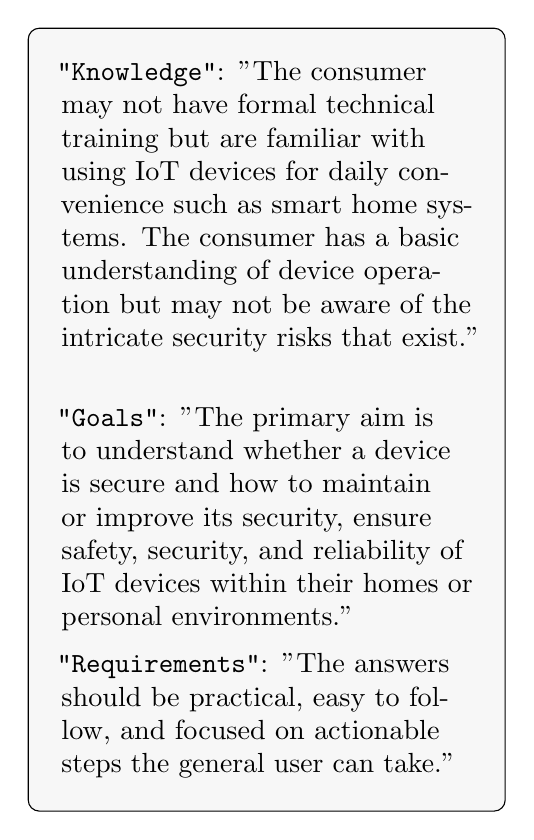
\begin{tikzpicture}
% Draw rounded rectangle with shadow
\node[rectangle, rounded corners, draw=black, fill=black!3!white, text width=0.43\textwidth, inner sep=12pt, align=left] (box) {
\textbf{\texttt{"Knowledge"}}: "The consumer may not have formal technical training but are familiar with using IoT devices for daily convenience such as smart home systems. The consumer has a basic understanding of device operation but may not be aware of the intricate security risks that exist."
\vspace{5pt}\\
\textbf{\texttt{"Goals"}}: "The primary aim is to understand whether a device is secure and how to maintain or improve its security, ensure safety, security, and reliability
of IoT devices within their homes or personal environments."
\vspace{5pt}\\
\textbf{\texttt{"Requirements"}}: "The answers should be practical, easy to follow, and focused on actionable steps the general user can take."
};
\end{tikzpicture}
}
\caption{The background for consumer utilized to guide the \chatiot\ to generate consumer-friendly outputs.}
\label{fig:usecasedef-consumer}
\end{figure}

\subsubsection{Guided Generation}\label{sec:resgen}

After retrieval, one direct step is feeding the retrieved documents and query to LLM to generate the answer. 
However, this simple approach is likely to result in user-unfriendly outputs. 
For example, consumers often lack the expertise needed to fully comprehend highly technical content, making such answers unhelpful and not actionable for them.

To address this issue, we incorporate user-specific backgrounds, including knowledge, goals, and requirements, into each user type's user-friendly prompt template \textit{UPT}. This adjustment guides LLM in generating answers tailored to the user's needs.
The specific background for the general consumer is shown in Figure~\ref{fig:usecasedef-consumer}, demonstrating how we simplify content for easy understanding. The background specifications of other user types can be referred to Appendix~\ref{appendix:bk}.


\begin{algorithm}[t]
\caption{\iotrgen}\label{alg:iotrgen}
\begin{algorithmic}[1]
\REQUIRE
User \textsf{role}, query $Q$, large language model $\mathcal{M}$, and retrievers $\{\mathcal{R}_i\}_{i=1}^n$.

\ENSURE
Generated answer $A$.

\STATE
\textcolor{gray}{$\triangleright$ \textbf{Procedure of Selector:}}

\STATE
Set prompt $\mathsf{SPT} = (\mathsf{Task}, \mathsf{role}, Q, \{\mathcal{R}_i\}_{i=1}^n)$, where $\mathsf{role}$ includes user's background implicitly and $\mathcal{R}_i$ indicates its description here.
\STATE
Inputting $\mathsf{SPT}$ to $\mathcal{M}$ and get $\{S_i\}_{i=1}^n = \mathcal{M}(\mathsf{SPT})$, where $S_i\in \{\mathsf{True}, \mathsf{False}\}$.

\STATE 
\textcolor{gray}{$\triangleright$ \textbf{Procedure of Self-Querying Retrieval:}}
\FORALL{$i=1, \dots, n$}
\IF{$\mathcal{S}_i = \mathsf{True}$}
\STATE
Execute self-querying retriever $\mathcal{R}_i$ and get documents $D_i=\mathcal{R}_i(Q)$
\ELSE
\STATE
Set $D_i = \mathsf{NULL}$.
\ENDIF
\ENDFOR

\STATE
\textcolor{gray}{$\triangleright$ \textbf{Procedure of Guided Generation:}}

\STATE
Set prompt $\mathsf{UPT} = (\mathsf{Task}, \mathsf{role}, Q, \{\mathcal{D}_i\}_{i=1}^n)$

\RETURN
$A = \mathcal{M}(\mathsf{UPT})$.


\end{algorithmic}
\end{algorithm}

Formally, we summarize and show the workflow of \iotrgen\ in algorithm~\ref{alg:iotrgen}.


\begin{figure*}
    \centering
    \includegraphics[width=\linewidth]{Figures/dataprocess.pdf}
    \caption{The construction of data processing toolkit \datakit. After collecting various IoT security datasets, \datakit\ first parses the raw data to get elements of multi-modal (step~\textcircled{1}), and then converts the multi-modal elements into text by utilizing LLM (step~\textcircled{2}). Finally, \datakit\ uses LLM to select fields for the page\_content and metadata of documents (step~\textcircled{3}), and optimizes the chunking strategy (step~\textcircled{4}).}
    \label{fig:dataprocess}
\end{figure*}

\subsection{Data Processing Toolkit}\label{sec:toolkit}

The raw data of the collected datasets are of different formats, \eg, PDF and JSON. These formats are not suitable for RAG processing directly, and thus we develop our end-to-end data processing \datakit. As shown in Figure~\ref{fig:dataprocess}, \datakit\ works in four steps:
\begin{itemize}
    \item[\ding{172}] \textbf{Parse Raw Data.} The initial step involves parsing raw data into distinct content elements such as text, tables, figures, and code. Leveraging existing tools like the unstructured library\footnote{\scriptsize \url{https://pypi.org/project/unstructured/}} helps in extracting textual content from threat reports, while the JSON library\footnote{\scriptsize \url{https://python.readthedocs.io/en/v2.7.2/library/json.html}} is useful for handling structured data from sources like VARIoT and MITRE ATT\&CK.
    
    \item[\ding{173}] \textbf{Convert Multi-Modal Elements to Text.} Once parsed, any multi-modal elements (\eg, tables, figures, code) must be converted into text descriptions for further processing. LLMs like LLaVA (for images)~\cite{liu2023llava,liu2023improvedllava,liu2024llavanext}, LLaMA3:8B (for tables), and CodeLlama (for code)~\cite{roziere2023code} are employed to generate these descriptions. This modular approach allows for easy integration of other LLMs to handle different types of multi-modal content.

    \item[\ding{174}] \textbf{Field Selection for Page\_Content \& Metadata.} In structured formats like JSON, content is often stored across multiple fields.
    Instead of using all fields, it is crucial to identify and utilize the most relevant ones for retrievers. This is done by sampling example items from each field and using an LLM (\eg, LLaMA3:8B) to intelligently select fields that best represent the document's page\_content and metadata, and the prompt is shown in Figure~\ref{fig:dataprocess}.
    Concretely, the selected fields for page\_content and metadata of each dataset are shown in \S~\ref{sec:exp-field}.

    \item[\ding{175}] \textbf{Optimize Chunking Strategy.} The final step involves selecting an appropriate chunking strategy, including the chunking size, overlap, and splitting method. The Ragas library~\cite{es2023ragas} is used to optimize this process, and the details are shown in algorithm~\ref{alg:chunkopt}.
\end{itemize}

\begin{algorithm}[t]
\caption{Optimize Chunking Strategy}\label{alg:chunkopt}
\begin{algorithmic}[1]
\REQUIRE
Documents $D$, chunking $sizes$, $overlaps$, and $splitters$ functions, $metrics=[precision, recall]$, and LLM $\mathcal{M}$.

\ENSURE
Optimized $(size^*, overlap^*, splitter^*)$.

\FORALL{$splitter \in splitters$}
\FORALL{$size \in chunk\_sizes$}
\FORALL{$overlap\in overlaps$}
\IF{$overlap < size$}
\STATE
\textcolor{gray}{$\triangleright$ \textbf{Split $D$ as small chunks:}}
\STATE
$\{d_i\}_i = splitter(D, size, overlap)$.
\STATE
$(p, r) = \text{Ragas.evaluate}(\{d_i\}_i, \mathcal{M}, metrics)$.
\ELSE
\STATE
\texttt{break.} \textcolor{gray}{$\triangleright$ \textbf{Go to next chunk size.}}
\ENDIF
\ENDFOR
\ENDFOR
\ENDFOR
\RETURN
chunking $(size^*, overlap^*, splitter^*)$ with a optimized trade-off between $(p, r)$.
\end{algorithmic}
\end{algorithm}

After obtaining the optimized chunking strategy, we split the documents into small chunks and use the all-MiniLM model for chunked text embedding. 
The documents are composed of chunked text, embedding, and metadata.
This approach ensures that the IoT security and threat datasets are processed efficiently and ready for further analysis or use in LLM. 
Note while many of these technologies are adapted from existing works, we foucs on putting them all together to develop an end-to-end data processing toolkit, which might be of independent interest and useful in practical applications.

\begin{table}[!hbpt]
    \centering
    \footnotesize
    \begin{tabular}{llp{0.4\linewidth}}
    \hline
         Use Case & Factor & Description \\
         \hline
         \multicolumn{3}{l}{\textbf{Professional Use Cases}}\\
         \quad Lawyer & Doctoral/Professional Degree & Advises clients on digital legal proceedings/transactions. \\
         \quad Elementary School Teacher & Bachelor’s degree & Teaches academic skills at the elementary school level. \\
         \quad IT Support Specialist & Some college, no degree & Maintains computer networks and provides technical help. \\
         \quad Government Eligibility Interviewer & High school diploma & Determine eligibility for government programs/resources. \\
         \quad Telemarketer & No formal education & Solicits donations or orders over the telephone. \\
         \hline
         \multicolumn{3}{l}{\textbf{Personal Use Cases}}\\
         \quad Digital Medical Advice & High Risk & Provide medical assessments prior to medical consultations. \\
         \quad Customized Lifestyle Coach & High / Limited Risk & Personalized advice for healthy living and wellness. \\
         \quad Personal Health Research & Limited Risk & Summarizes research related to personal health issues. \\
         \quad Nutrition Optimizer & Limited / Low Risk & Personalize meals and optimize nutritional intake. \\
         \quad Flavorful Swaps & Low Risk & Suggest delicious and healthy alternatives food options. \\
    \hline
    \end{tabular}
    \caption{Use cases selected for our study by categories. Use case descriptions were shortened for brevity.}
    \label{tab:use-cases}
\end{table}



\section{Experiments}
\label{sec:exp}
Following the settings in Section \ref{sec:existing}, we evaluate \textit{NovelSum}'s correlation with the fine-tuned model performance across 53 IT datasets and compare it with previous diversity metrics. Additionally, we conduct a correlation analysis using Qwen-2.5-7B \cite{yang2024qwen2} as the backbone model, alongside previous LLaMA-3-8B experiments, to further demonstrate the metric's effectiveness across different scenarios. Qwen is used for both instruction tuning and deriving semantic embeddings. Due to resource constraints, we run each strategy on Qwen for two rounds, resulting in 25 datasets. 

\subsection{Main Results}

\begin{table*}[!t]
    \centering
    \resizebox{\linewidth}{!}{
    \begin{tabular}{lcccccccccc}
    \toprule
    \multirow{3}*{\textbf{Diversity Metrics}} & \multicolumn{10}{c}{\textbf{Data Selection Strategies}} \\
    \cmidrule(lr){2-11}
    & \multirow{2}*{\textbf{K-means}} & \multirow{2}*{\vtop{\hbox{\textbf{K-Center}}\vspace{1mm}\hbox{\textbf{-Greedy}}}}  & \multirow{2}*{\textbf{QDIT}} & \multirow{2}*{\vtop{\hbox{\textbf{Repr}}\vspace{1mm}\hbox{\textbf{Filter}}}} & \multicolumn{5}{c}{\textbf{Random}} & \multirow{2}{*}{\textbf{Duplicate}} \\ 
    \cmidrule(lr){6-10}
    & & & & & \textbf{$\mathcal{X}^{all}$} & ShareGPT & WizardLM & Alpaca & Dolly &  \\
    \midrule
    \rowcolor{gray!15} \multicolumn{11}{c}{\textit{LLaMA-3-8B}} \\
    Facility Loc. $_{\times10^5}$ & \cellcolor{BLUE!40} 2.99 & \cellcolor{ORANGE!10} 2.73 & \cellcolor{BLUE!40} 2.99 & \cellcolor{BLUE!20} 2.86 & \cellcolor{BLUE!40} 2.99 & \cellcolor{BLUE!0} 2.83 & \cellcolor{BLUE!30} 2.88 & \cellcolor{BLUE!0} 2.83 & \cellcolor{ORANGE!20} 2.59 & \cellcolor{ORANGE!30} 2.52 \\    
    DistSum$_{cosine}$  & \cellcolor{BLUE!30} 0.648 & \cellcolor{BLUE!60} 0.746 & \cellcolor{BLUE!0} 0.629 & \cellcolor{BLUE!50} 0.703 & \cellcolor{BLUE!10} 0.634 & \cellcolor{BLUE!40} 0.656 & \cellcolor{ORANGE!30} 0.578 & \cellcolor{ORANGE!10} 0.605 & \cellcolor{ORANGE!20} 0.603 & \cellcolor{BLUE!10} 0.634 \\
    Vendi Score $_{\times10^7}$ & \cellcolor{BLUE!30} 1.70 & \cellcolor{BLUE!60} 2.53 & \cellcolor{BLUE!10} 1.59 & \cellcolor{BLUE!50} 2.23 & \cellcolor{BLUE!20} 1.61 & \cellcolor{BLUE!30} 1.70 & \cellcolor{ORANGE!10} 1.44 & \cellcolor{ORANGE!20} 1.32 & \cellcolor{ORANGE!10} 1.44 & \cellcolor{ORANGE!30} 0.05 \\
    \textbf{NovelSum (Ours)} & \cellcolor{BLUE!60} 0.693 & \cellcolor{BLUE!50} 0.687 & \cellcolor{BLUE!30} 0.673 & \cellcolor{BLUE!20} 0.671 & \cellcolor{BLUE!40} 0.675 & \cellcolor{BLUE!10} 0.628 & \cellcolor{BLUE!0} 0.591 & \cellcolor{ORANGE!10} 0.572 & \cellcolor{ORANGE!20} 0.50 & \cellcolor{ORANGE!30} 0.461 \\
    \midrule    
    \textbf{Model Performance} & \cellcolor{BLUE!60}1.32 & \cellcolor{BLUE!50}1.31 & \cellcolor{BLUE!40}1.25 & \cellcolor{BLUE!30}1.05 & \cellcolor{BLUE!20}1.20 & \cellcolor{BLUE!10}0.83 & \cellcolor{BLUE!0}0.72 & \cellcolor{ORANGE!10}0.07 & \cellcolor{ORANGE!20}-0.14 & \cellcolor{ORANGE!30}-1.35 \\
    \midrule
    \midrule
    \rowcolor{gray!15} \multicolumn{11}{c}{\textit{Qwen-2.5-7B}} \\
    Facility Loc. $_{\times10^5}$ & \cellcolor{BLUE!40} 3.54 & \cellcolor{ORANGE!30} 3.42 & \cellcolor{BLUE!40} 3.54 & \cellcolor{ORANGE!20} 3.46 & \cellcolor{BLUE!40} 3.54 & \cellcolor{BLUE!30} 3.51 & \cellcolor{BLUE!10} 3.50 & \cellcolor{BLUE!10} 3.50 & \cellcolor{ORANGE!20} 3.46 & \cellcolor{BLUE!0} 3.48 \\ 
    DistSum$_{cosine}$ & \cellcolor{BLUE!30} 0.260 & \cellcolor{BLUE!60} 0.440 & \cellcolor{BLUE!0} 0.223 & \cellcolor{BLUE!50} 0.421 & \cellcolor{BLUE!10} 0.230 & \cellcolor{BLUE!40} 0.285 & \cellcolor{ORANGE!20} 0.211 & \cellcolor{ORANGE!30} 0.189 & \cellcolor{ORANGE!10} 0.221 & \cellcolor{BLUE!20} 0.243 \\
    Vendi Score $_{\times10^6}$ & \cellcolor{ORANGE!10} 1.60 & \cellcolor{BLUE!40} 3.09 & \cellcolor{BLUE!10} 2.60 & \cellcolor{BLUE!60} 7.15 & \cellcolor{ORANGE!20} 1.41 & \cellcolor{BLUE!50} 3.36 & \cellcolor{BLUE!20} 2.65 & \cellcolor{BLUE!0} 1.89 & \cellcolor{BLUE!30} 3.04 & \cellcolor{ORANGE!30} 0.20 \\
    \textbf{NovelSum (Ours)}  & \cellcolor{BLUE!40} 0.440 & \cellcolor{BLUE!60} 0.505 & \cellcolor{BLUE!20} 0.403 & \cellcolor{BLUE!50} 0.495 & \cellcolor{BLUE!30} 0.408 & \cellcolor{BLUE!10} 0.392 & \cellcolor{BLUE!0} 0.349 & \cellcolor{ORANGE!10} 0.336 & \cellcolor{ORANGE!20} 0.320 & \cellcolor{ORANGE!30} 0.309 \\
    \midrule
    \textbf{Model Performance} & \cellcolor{BLUE!30} 1.06 & \cellcolor{BLUE!60} 1.45 & \cellcolor{BLUE!40} 1.23 & \cellcolor{BLUE!50} 1.35 & \cellcolor{BLUE!20} 0.87 & \cellcolor{BLUE!10} 0.07 & \cellcolor{BLUE!0} -0.08 & \cellcolor{ORANGE!10} -0.38 & \cellcolor{ORANGE!30} -0.49 & \cellcolor{ORANGE!20} -0.43 \\
    \bottomrule
    \end{tabular}
    }
    \caption{Measuring the diversity of datasets selected by different strategies using \textit{NovelSum} and baseline metrics. Fine-tuned model performances (Eq. \ref{eq:perf}), based on MT-bench and AlpacaEval, are also included for cross reference. Darker \colorbox{BLUE!60}{blue} shades indicate higher values for each metric, while darker \colorbox{ORANGE!30}{orange} shades indicate lower values. While data selection strategies vary in performance on LLaMA-3-8B and Qwen-2.5-7B, \textit{NovelSum} consistently shows a stronger correlation with model performance than other metrics. More results are provided in Appendix \ref{app:results}.}
    \label{tbl:main}
    \vspace{-4mm}
\end{table*}


\begin{table}[t!]
\centering
\resizebox{\linewidth}{!}{
\begin{tabular}{lcccc}
\toprule
\multirow{2}*{\textbf{Diversity Metrics}} & \multicolumn{3}{c}{\textbf{LLaMA}} & \textbf{Qwen}\\
\cmidrule(lr){2-4} \cmidrule(lr){5-5} 
& \textbf{Pearson} & \textbf{Spearman} & \textbf{Avg.} & \textbf{Avg.} \\
\midrule
TTR & -0.38 & -0.16 & -0.27 & -0.30 \\
vocd-D & -0.43 & -0.17 & -0.30 & -0.31 \\
\midrule
Facility Loc. & 0.86 & 0.69 & 0.77 & 0.08 \\
Entropy & 0.93 & 0.80 & 0.86 & 0.63 \\
\midrule
LDD & 0.61 & 0.75 & 0.68 & 0.60 \\
KNN Distance & 0.59 & 0.80 & 0.70 & 0.67 \\
DistSum$_{cosine}$ & 0.85 & 0.67 & 0.76 & 0.51 \\
Vendi Score & 0.70 & 0.85 & 0.78 & 0.60 \\
DistSum$_{L2}$ & 0.86 & 0.76 & 0.81 & 0.51 \\
Cluster Inertia & 0.81 & 0.85 & 0.83 & 0.76 \\
Radius & 0.87 & 0.81 & 0.84 & 0.48 \\
\midrule
NovelSum & \textbf{0.98} & \textbf{0.95} & \textbf{0.97} & \textbf{0.90} \\
\bottomrule
\end{tabular}
}
\caption{Correlations between different metrics and model performance on LLaMA-3-8B and Qwen-2.5-7B.  “Avg.” denotes the average correlation (Eq. \ref{eq:cor}).}
\label{tbl:correlations}
\vspace{-2mm}
\end{table}

\paragraph{\textit{NovelSum} consistently achieves state-of-the-art correlation with model performance across various data selection strategies, backbone LLMs, and correlation measures.}
Table \ref{tbl:main} presents diversity measurement results on datasets constructed by mainstream data selection methods (based on $\mathcal{X}^{all}$), random selection from various sources, and duplicated samples (with only $m=100$ unique samples). 
Results from multiple runs are averaged for each strategy.
Although these strategies yield varying performance rankings across base models, \textit{NovelSum} consistently tracks changes in IT performance by accurately measuring dataset diversity. For instance, K-means achieves the best performance on LLaMA with the highest NovelSum score, while K-Center-Greedy excels on Qwen, also correlating with the highest NovelSum. Table \ref{tbl:correlations} shows the correlation coefficients between various metrics and model performance for both LLaMA and Qwen experiments, where \textit{NovelSum} achieves state-of-the-art correlation across different models and measures.

\paragraph{\textit{NovelSum} can provide valuable guidance for data engineering practices.}
As a reliable indicator of data diversity, \textit{NovelSum} can assess diversity at both the dataset and sample levels, directly guiding data selection and construction decisions. For example, Table \ref{tbl:main} shows that the combined data source $\mathcal{X}^{all}$ is a better choice for sampling diverse IT data than other sources. Moreover, \textit{NovelSum} can offer insights through comparative analyses, such as: (1) ShareGPT, which collects data from real internet users, exhibits greater diversity than Dolly, which relies on company employees, suggesting that IT samples from diverse sources enhance dataset diversity \cite{wang2024diversity-logD}; (2) In LLaMA experiments, random selection can outperform some mainstream strategies, aligning with prior work \cite{xia2024rethinking,diddee2024chasing}, highlighting gaps in current data selection methods for optimizing diversity.



\subsection{Ablation Study}


\textit{NovelSum} involves several flexible hyperparameters and variations. In our main experiments, \textit{NovelSum} uses cosine distance to compute $d(x_i, x_j)$ in Eq. \ref{eq:dad}. We set $\alpha = 1$, $\beta = 0.5$, and $K = 10$ nearest neighbors in Eq. \ref{eq:pws} and \ref{eq:dad}. Here, we conduct an ablation study to investigate the impact of these settings based on LLaMA-3-8B.

\begin{table}[ht!]
\centering
\resizebox{\linewidth}{!}{
\begin{tabular}{lccc}
\toprule
\textbf{Variants} & \textbf{Pearson} & \textbf{Spearman} & \textbf{Avg.} \\
\midrule
NovelSum & 0.98 & 0.96 & 0.97 \\
\midrule
\hspace{0.10cm} - Use $L2$ distance & 0.97 & 0.83 & 0.90\textsubscript{↓ 0.08} \\
\hspace{0.10cm} - $K=20$ & 0.98 & 0.96 & 0.97\textsubscript{↓ 0.00} \\
\hspace{0.10cm} - $\alpha=0$ (w/o proximity) & 0.79 & 0.31 & 0.55\textsubscript{↓ 0.42} \\
\hspace{0.10cm} - $\alpha=2$ & 0.73 & 0.88 & 0.81\textsubscript{↓ 0.16} \\
\hspace{0.10cm} - $\beta=0$ (w/o density) & 0.92 & 0.89 & 0.91\textsubscript{↓ 0.07} \\
\hspace{0.10cm} - $\beta=1$ & 0.90 & 0.62 & 0.76\textsubscript{↓ 0.21} \\
\bottomrule
\end{tabular}
}
\caption{Ablation Study for \textit{NovelSum}.}
\label{tbl:ablation}
\vspace{-2mm}
\end{table}

In Table \ref{tbl:ablation}, $\alpha=0$ removes the proximity weights, and $\beta=0$ eliminates the density multiplier. We observe that both $\alpha=0$ and $\beta=0$ significantly weaken the correlation, validating the benefits of the proximity-weighted sum and density-aware distance. Additionally, improper values for $\alpha$ and $\beta$ greatly reduce the metric's reliability, highlighting that \textit{NovelSum} strikes a delicate balance between distances and distribution. Replacing cosine distance with Euclidean distance and using more neighbors for density approximation have minimal impact, particularly on Pearson's correlation, demonstrating \textit{NovelSum}'s robustness to different distance measures.







Our work draws heavily from the literature on semiparametric inference and double machine learning~\citep{robins1994estimation,robins1995semiparametric,tsiatis2006semiparametric,chernozhukov2018double}. In particular, our estimator is an optimal combination of several Augmented Inverse Probability Weighting~(\aipw) estimators, whose outcome regressions are replaced with foundation models. Importantly, the standard $\aipw$ estimator, which relies on an outcome regression estimated using experimental data alone, is also included in the combination. This approach allows \ours~to significantly reduce finite sample (and potentially asymptotic) variance while attaining the semiparametric \emph{efficiency bound}---the smallest asymptotic variance among all consistent and asymptotically normal estimators of the average treatment effect---even when the foundation models are arbitrarily biased.


\paragraph{Integrating foundation models}
Prediction-powered inference~(\ppi)~\citep{angelopoulos2023prediction} is a statistical framework that constructs valid confidence intervals using a small labeled dataset and a large unlabeled dataset imputed by a foundation model. $\ppi$ has been applied in various domains, including generalization of causal inferences~\citep{demirel24prediction}, large language model evaluation~\citep{fisch2024stratified,dorner2024limitsscalableevaluationfrontier}, and improving the efficiency of social science experiments~\citep{broskamixed,egami2024using}. However, unlike our approach, $\ppi$ requires access to an additional unlabeled dataset from the same distribution as the experimental sample, which may be as costly as labeled data. Recent work by \citet{poulet2025prediction} introduces 
Prediction-powered inference for clinical trials ($\ppct$), an adaptation of $\ppi$ to estimate  average treatment effects in randomized experiments without any additional  external data. $\ppct$ combines the difference in means estimator with an 
$\aipw$ estimator that integrates the same foundation model as the outcome regression for both treatment and control groups. However, our work differs in two key aspects:
(i) $\ppct$ integrates a single foundation model, and (ii) $\ppct$ does not include the standard $\aipw$ estimator with the outcome regression estimated from experimental data. As a result, $\ppct$ cannot achieve the efficiency bound unless the foundation model is almost surely equal to the underlying outcome regression. 


 



\paragraph{Integrating observational data} There is growing interest in augmenting randomized experiments with data from observational studies to improve statistical precision. One approach involves first testing whether the observational data is compatible with the experimental data~\citep{dahabreh2024using}---for instance, using a statistical test to assess if the mean of the outcome conditional on the covariates is invariant across studies \cite{luedtke2019omnibus,hussain2023falsification,de2024detecting}—and then combining the datasets to improve precision, if the test does not reject. These tests, however, have low statistical power, especially when the experimental sample size is small, which is precisely when leveraging observational data would be most beneficial. To overcome this, a recent line of work integrates a prognostic score estimated from observational data as a covariate when estimating the outcome regression~\citep{schuler2022increasing,liao2023prognostic}. However, increasing the dimensionality of the problem---by adding an additional covariate---can increase estimation error and inflate the finite sample variance. Finally, the work most closely related to ours is \citet{karlsson2024robust}, that integrates an outcome regression estimated from observational data into the \aipw~estimator. In contrast, our approach is not constrained by the availability of well-structured observational data, since it leverages black-box foundation models trained on external data sources.

\section{Conclusion}
In this work, we propose a simple yet effective approach, called SMILE, for graph few-shot learning with fewer tasks. Specifically, we introduce a novel dual-level mixup strategy, including within-task and across-task mixup, for enriching the diversity of nodes within each task and the diversity of tasks. Also, we incorporate the degree-based prior information to learn expressive node embeddings. Theoretically, we prove that SMILE effectively enhances the model's generalization performance. Empirically, we conduct extensive experiments on multiple benchmarks and the results suggest that SMILE significantly outperforms other baselines, including both in-domain and cross-domain few-shot settings.

\section*{Acknowledgements} This research is supported by the National Research Foundation, Singapore, under its National Satellite of Excellence Programme “Design Science and Technology for Secure Critical Infrastructure: Phase II” (Award No: NRF-NCR25-NSOE05-0001). Any opinions, findings and conclusions or recommendations expressed in this material are those of the author(s) and do not reflect the views of National Research Foundation, Singapore.



\begin{thebibliography}{00}

\bibitem{kouicem2018internet}
D.~E. Kouicem, A.~Bouabdallah, and H.~Lakhlef, ``Internet of things security: A top-down survey,'' \emph{Computer Networks}, vol. 141, pp. 199--221, 2018.

\bibitem{ahmad2021machine}
R.~Ahmad and I.~Alsmadi, ``Machine learning approaches to iot security: A systematic literature review,'' \emph{Internet of Things}, vol.~14, p. 100365, 2021.

\bibitem{williams2017identifying}
R.~Williams, E.~McMahon, S.~Samtani, M.~Patton, and H.~Chen, ``Identifying vulnerabilities of consumer internet of things (iot) devices: A scalable approach,'' in \emph{2017 IEEE International Conference on Intelligence and Security Informatics (ISI)}.\hskip 1em plus 0.5em minus 0.4em\relax IEEE, 2017, pp. 179--181.

\bibitem{deogirikar2017security}
J.~Deogirikar and A.~Vidhate, ``Security attacks in iot: A survey,'' in \emph{2017 International Conference on I-SMAC (IoT in Social, Mobile, Analytics and Cloud)(I-SMAC)}.\hskip 1em plus 0.5em minus 0.4em\relax IEEE, 2017, pp. 32--37.

\bibitem{gormucs2018security}
S.~G{\"o}rm{\"u}{\c{s}}, H.~Ayd{\i}n, and G.~Uluta{\c{s}}, ``Security for the internet of things: a survey of existing mechanisms, protocols and open research issues,'' \emph{Journal of the Faculty of Engineering and Architecture of Gazi University}, vol.~33, no.~4, pp. 1247--1272, 2018.

\bibitem{sokiotllm}
M.~A. Ferrag, M.~Ndhlovu, N.~Tihanyi, L.~C. Cordeiro, M.~Debbah, T.~Lestable, and N.~S. Thandi, ``Revolutionizing cyber threat detection with large language models: A privacy-preserving bert-based lightweight model for iot/iiot devices,'' \emph{IEEE Access}, vol.~12, pp. 23\,733--23\,750, 2024.

\bibitem{ma}
X.~Ma, L.~Luo, and Q.~Zeng, ``From one thousand pages of specification to unveiling hidden bugs: Large language model assisted fuzzing of matter {IoT} devices,'' in \emph{33rd USENIX Security Symposium (USENIX Security 24)}.\hskip 1em plus 0.5em minus 0.4em\relax Philadelphia, PA: USENIX Association, Aug. 2024, pp. 4783--4800. [Online]. Available: \url{https://www.usenix.org/conference/usenixsecurity24/presentation/ma-xiaoyue}

\bibitem{llmiotfuz}
J.~Wang, L.~Yu, and X.~Luo, ``Llmif: Augmented large language model for fuzzing iot devices,'' in \emph{2024 IEEE Symposium on Security and Privacy (SP)}.\hskip 1em plus 0.5em minus 0.4em\relax Los Alamitos, CA, USA: IEEE Computer Society, may 2024, pp. 881--896. [Online]. Available: \url{https://doi.ieeecomputersociety.org/10.1109/SP54263.2024.00211}

\bibitem{yang2023iot}
Y.~Yang, ``Iot software vulnerability detection techniques through large language model,'' in \emph{International Conference on Formal Engineering Methods}.\hskip 1em plus 0.5em minus 0.4em\relax Springer, 2023, pp. 285--290.

\bibitem{mo2024iot}
S.~Mo, R.~Salakhutdinov, L.-P. Morency, and P.~P. Liang, ``Iot-lm: Large multisensory language models for the internet of things,'' \emph{arXiv preprint arXiv:2407.09801}, 2024.

\bibitem{meyuhas2024iotlabel}
B.~Meyuhas, A.~Bremler-Barr, and T.~Shapira, ``Iot device labeling using large language models,'' \emph{arXiv preprint arXiv:2403.01586}, 2024.

\bibitem{llmiotcontrol}
B.~Rong and H.~Rutagemwa, ``Leveraging large language models for intelligent control of 6g integrated tn-ntn with iot service,'' \emph{IEEE Network}, vol.~38, no.~4, pp. 136--142, 2024.

\bibitem{ferraris2024ici}
D.~Ferraris, K.~Kotis, and C.~Kalloniatis, ``Enhancing trustapis methodology in the web of things with llm-generated iot trust semantics,'' in \emph{26th International Conference on Information and Communications Security (ICICS 2024)}.\hskip 1em plus 0.5em minus 0.4em\relax Mytilene, Lesvos, Greece: Springer, 2024. [Online]. Available: \url{/wp-content/papers/ferraris2024ici.pdf}

\bibitem{CVE_Mission}
{CVE Program}, ``{CVE\textsuperscript{\textregistered} Program Mission},'' \url{https://www.cve.org/}, n.d.

\bibitem{VARIoT_db}
M.~Janiszewski, A.~Felkner, P.~Lewandowski, M.~Rytel, and H.~Romanowski, ``Automatic actionable information processing and trust management towards safer internet of things,'' \emph{Sensors}, vol.~21, no.~13, 2021. [Online]. Available: \url{https://www.mdpi.com/1424-8220/21/13/4359}

\bibitem{strom2018mitre}
B.~E. Strom, A.~Applebaum, D.~P. Miller, K.~C. Nickels, A.~G. Pennington, and C.~B. Thomas, ``Mitre att\&ck: Design and philosophy,'' in \emph{Technical report}.\hskip 1em plus 0.5em minus 0.4em\relax The MITRE Corporation, 2018.

\bibitem{abdul2019comprehensive}
H.~A. Abdul-Ghani and D.~Konstantas, ``A comprehensive study of security and privacy guidelines, threats, and countermeasures: An iot perspective,'' \emph{Journal of Sensor and Actuator Networks}, vol.~8, no.~2, p.~22, 2019.

\bibitem{wright2022regulating}
E.~Wright, D.~Lindsay, and G.~Wilkinson, ``Regulating to protect security and privacy in the internet of things (iot): Draft report,'' 2022.

\bibitem{es2023ragas}
S.~Es, J.~James, L.~Espinosa-Anke, and S.~Schockaert, ``Ragas: Automated evaluation of retrieval augmented generation,'' \emph{arXiv preprint arXiv:2309.15217}, 2023.

\bibitem{dragomir2016survey}
D.~Dragomir, L.~Gheorghe, S.~Costea, and A.~Radovici, ``A survey on secure communication protocols for iot systems,'' in \emph{2016 international workshop on Secure Internet of Things (SIoT)}.\hskip 1em plus 0.5em minus 0.4em\relax IEEE, 2016, pp. 47--62.

\bibitem{alrawi2021circle}
O.~Alrawi, C.~Lever, K.~Valakuzhy, K.~Snow, F.~Monrose, M.~Antonakakis \emph{et~al.}, ``The circle of life: A $\{$large-scale$\}$ study of the $\{$IoT$\}$ malware lifecycle,'' in \emph{30th USENIX Security Symposium (USENIX Security 21)}, 2021, pp. 3505--3522.

\bibitem{iacovazzi2023towards}
A.~Iacovazzi, H.~Wang, I.~Butun, and S.~Raza, ``Towards cyber threat intelligence for the iot,'' in \emph{2023 19th International Conference on Distributed Computing in Smart Systems and the Internet of Things (DCOSS-IoT)}.\hskip 1em plus 0.5em minus 0.4em\relax IEEE, 2023, pp. 483--490.

\bibitem{bou2020cyber}
E.~Bou-Harb and N.~Neshenko, \emph{Cyber threat intelligence for the internet of things}.\hskip 1em plus 0.5em minus 0.4em\relax Springer, 2020.

\bibitem{wagner2019cyber}
T.~D. Wagner, K.~Mahbub, E.~Palomar, and A.~E. Abdallah, ``Cyber threat intelligence sharing: Survey and research directions,'' \emph{Computers \& Security}, vol.~87, p. 101589, 2019.

\bibitem{saurabh2024hms}
K.~Saurabh, V.~Sharma, U.~Singh, R.~Khondoker, R.~Vyas, and O.~Vyas, ``Hms-ids: Threat intelligence integration for zero-day exploits and advanced persistent threats in iiot,'' \emph{Arabian Journal for Science and Engineering}, pp. 1--21, 2024.

\bibitem{ahmed2023securing}
S.~Ahmed and M.~Khan, ``Securing the internet of things (iot): A comprehensive study on the intersection of cybersecurity, privacy, and connectivity in the iot ecosystem,'' \emph{AI, IoT and the Fourth Industrial Revolution Review}, vol.~13, no.~9, pp. 1--17, 2023.

\bibitem{gpt}
A.~Radford and K.~Narasimhan, ``Improving language understanding by generative pre-training,'' 2018.

\bibitem{zhuge2021kaleido}
M.~Zhuge, D.~Gao, D.-P. Fan, L.~Jin, B.~Chen, H.~Zhou, M.~Qiu, and L.~Shao, ``Kaleido-bert: Vision-language pre-training on fashion domain,'' in \emph{Proceedings of the IEEE/CVF Conference on Computer Vision and Pattern Recognition}, 2021, pp. 12\,647--12\,657.

\bibitem{docformer}
S.~Appalaraju, B.~Jasani, B.~U. Kota, Y.~Xie, and R.~Manmatha, ``Docformer: End-to-end transformer for document understanding,'' in \emph{Proceedings of the IEEE/CVF international conference on computer vision}, 2021, pp. 993--1003.

\bibitem{kim2022ocr}
G.~Kim, T.~Hong, M.~Yim, J.~Nam, J.~Park, J.~Yim, W.~Hwang, S.~Yun, D.~Han, and S.~Park, ``Ocr-free document understanding transformer,'' in \emph{European Conference on Computer Vision}.\hskip 1em plus 0.5em minus 0.4em\relax Springer, 2022, pp. 498--517.

\bibitem{fan2024survey}
W.~Fan, Y.~Ding, L.~Ning, S.~Wang, H.~Li, D.~Yin, T.-S. Chua, and Q.~Li, ``A survey on rag meeting llms: Towards retrieval-augmented large language models,'' in \emph{Proceedings of the 30th ACM SIGKDD Conference on Knowledge Discovery and Data Mining}, 2024, pp. 6491--6501.

\bibitem{lewis2020retrieval}
P.~Lewis, E.~Perez, A.~Piktus, F.~Petroni, V.~Karpukhin, N.~Goyal, H.~K{\"u}ttler, M.~Lewis, W.-t. Yih, T.~Rockt{\"a}schel \emph{et~al.}, ``Retrieval-augmented generation for knowledge-intensive nlp tasks,'' \emph{Advances in Neural Information Processing Systems}, vol.~33, pp. 9459--9474, 2020.

\bibitem{liu2023llava}
H.~Liu, C.~Li, Q.~Wu, and Y.~J. Lee, ``Visual instruction tuning,'' 2023.

\bibitem{liu2023improvedllava}
H.~Liu, C.~Li, Y.~Li, and Y.~J. Lee, ``Improved baselines with visual instruction tuning,'' 2023.

\bibitem{liu2024llavanext}
H.~Liu, C.~Li, Y.~Li, B.~Li, Y.~Zhang, S.~Shen, and Y.~J. Lee, ``Llava-next: Improved reasoning, ocr, and world knowledge,'' January 2024. [Online]. Available: \url{https://llava-vl.github.io/blog/2024-01-30-llava-next/}

\bibitem{roziere2023code}
B.~Roziere, J.~Gehring, F.~Gloeckle, S.~Sootla, I.~Gat, X.~E. Tan, Y.~Adi, J.~Liu, R.~Sauvestre, T.~Remez \emph{et~al.}, ``Code llama: Open foundation models for code,'' \emph{arXiv preprint arXiv:2308.12950}, 2023.

\bibitem{elasticsearch2018elasticsearch}
``Elasticsearch,'' \emph{software, version}, vol.~6, no.~1, 2018.

\bibitem{docker-desktop}
``Docker desktop, version 4.29.0,'' \url{https://www.docker.com/products/docker-desktop}, 2024.

\bibitem{langchain2024}
``Langchain,'' \url{https://github.com/langchain-ai/langchain}, 2024, version 0.2.5.

\bibitem{streamlit}
``Streamlit, version 1.33.0,'' \url{https://streamlit.io}, 2024, accessed: 2024-09-02.

\bibitem{luo2022transformer}
Y.~Luo, X.~Chen, N.~Ge, W.~Feng, and J.~Lu, ``Transformer-based malicious traffic detection for internet of things,'' in \emph{ICC 2022-IEEE International Conference on Communications}.\hskip 1em plus 0.5em minus 0.4em\relax IEEE, 2022, pp. 4187--4192.

\bibitem{shafiq2020corrauc}
M.~Shafiq, Z.~Tian, A.~K. Bashir, X.~Du, and M.~Guizani, ``Corrauc: a malicious bot-iot traffic detection method in iot network using machine-learning techniques,'' \emph{IEEE Internet of Things Journal}, vol.~8, no.~5, pp. 3242--3254, 2020.

\bibitem{vasan2020mthael}
D.~Vasan, M.~Alazab, S.~Venkatraman, J.~Akram, and Z.~Qin, ``Mthael: Cross-architecture iot malware detection based on neural network advanced ensemble learning,'' \emph{IEEE Transactions on Computers}, vol.~69, no.~11, pp. 1654--1667, 2020.

\bibitem{chaganti2022deep}
R.~Chaganti, V.~Ravi, and T.~D. Pham, ``Deep learning based cross architecture internet of things malware detection and classification,'' \emph{Computers \& Security}, vol. 120, p. 102779, 2022.

\bibitem{aung2022atlas}
Y.~L. Aung, M.~Ochoa, and J.~Zhou, ``Atlas: A practical attack detection and live malware analysis system for iot threat intelligence,'' in \emph{International Conference on Information Security}.\hskip 1em plus 0.5em minus 0.4em\relax Springer, 2022, pp. 319--338.

\bibitem{neshenko2019demystifying}
N.~Neshenko, E.~Bou-Harb, J.~Crichigno, G.~Kaddoum, and N.~Ghani, ``Demystifying iot security: An exhaustive survey on iot vulnerabilities and a first empirical look on internet-scale iot exploitations,'' \emph{IEEE Communications Surveys \& Tutorials}, vol.~21, no.~3, pp. 2702--2733, 2019.

\bibitem{al2020survey}
M.~A. Al-Garadi, A.~Mohamed, A.~K. Al-Ali, X.~Du, I.~Ali, and M.~Guizani, ``A survey of machine and deep learning methods for internet of things (iot) security,'' \emph{IEEE communications surveys \& tutorials}, vol.~22, no.~3, pp. 1646--1685, 2020.

\bibitem{otoum2022dl}
Y.~Otoum, D.~Liu, and A.~Nayak, ``Dl-ids: a deep learning--based intrusion detection framework for securing iot,'' \emph{Transactions on Emerging Telecommunications Technologies}, vol.~33, no.~3, p. e3803, 2022.

\bibitem{tambe2019detection}
A.~Tambe, Y.~L. Aung, R.~Sridharan, M.~Ochoa, N.~O. Tippenhauer, A.~Shabtai, and Y.~Elovici, ``Detection of threats to iot devices using scalable vpn-forwarded honeypots,'' in \emph{Proceedings of the Ninth ACM Conference on Data and Application Security and Privacy}, 2019, pp. 85--96.

\bibitem{ji2024sevenllm}
H.~Ji, J.~Yang, L.~Chai, C.~Wei, L.~Yang, Y.~Duan, Y.~Wang, T.~Sun, H.~Guo, T.~Li \emph{et~al.}, ``Sevenllm: Benchmarking, eliciting, and enhancing abilities of large language models in cyber threat intelligence,'' \emph{arXiv preprint arXiv:2405.03446}, 2024.

\bibitem{llmtikg}
Y.~Hu, F.~Zou, J.~Han, X.~Sun, and Y.~Wang, ``Llm-tikg: Threat intelligence knowledge graph construction utilizing large language model,'' \emph{Computers \& Security}, vol. 145, p. 103999, 2024.

\bibitem{ferraris2020trustapis}
D.~Ferraris and C.~Fernandez-Gago, ``Trustapis: a trust requirements elicitation method for iot,'' \emph{International Journal of Information Security}, vol.~19, no.~1, pp. 111--127, 2020.

\bibitem{cui2024llmind}
H.~Cui, Y.~Du, Q.~Yang, Y.~Shao, and S.~C. Liew, ``Llmind: Orchestrating ai and iot with llm for complex task execution,'' \emph{IEEE Communications Magazine}, 2024.

\bibitem{xu2024penetrative}
H.~Xu, L.~Han, Q.~Yang, M.~Li, and M.~Srivastava, ``Penetrative ai: Making llms comprehend the physical world,'' in \emph{Proceedings of the 25th International Workshop on Mobile Computing Systems and Applications}, 2024, pp. 1--7.

\bibitem{deldari2024auditnet}
S.~Deldari, M.~Goudarzi, A.~Joshi, A.~Shaghaghi, S.~Finn, F.~D. Salim, and S.~Jha, ``Auditnet: A conversational ai-based security assistant,'' \emph{arXiv preprint arXiv:2407.14116}, 2024.

\end{thebibliography}





\subsection{Lloyd-Max Algorithm}
\label{subsec:Lloyd-Max}
For a given quantization bitwidth $B$ and an operand $\bm{X}$, the Lloyd-Max algorithm finds $2^B$ quantization levels $\{\hat{x}_i\}_{i=1}^{2^B}$ such that quantizing $\bm{X}$ by rounding each scalar in $\bm{X}$ to the nearest quantization level minimizes the quantization MSE. 

The algorithm starts with an initial guess of quantization levels and then iteratively computes quantization thresholds $\{\tau_i\}_{i=1}^{2^B-1}$ and updates quantization levels $\{\hat{x}_i\}_{i=1}^{2^B}$. Specifically, at iteration $n$, thresholds are set to the midpoints of the previous iteration's levels:
\begin{align*}
    \tau_i^{(n)}=\frac{\hat{x}_i^{(n-1)}+\hat{x}_{i+1}^{(n-1)}}2 \text{ for } i=1\ldots 2^B-1
\end{align*}
Subsequently, the quantization levels are re-computed as conditional means of the data regions defined by the new thresholds:
\begin{align*}
    \hat{x}_i^{(n)}=\mathbb{E}\left[ \bm{X} \big| \bm{X}\in [\tau_{i-1}^{(n)},\tau_i^{(n)}] \right] \text{ for } i=1\ldots 2^B
\end{align*}
where to satisfy boundary conditions we have $\tau_0=-\infty$ and $\tau_{2^B}=\infty$. The algorithm iterates the above steps until convergence.

Figure \ref{fig:lm_quant} compares the quantization levels of a $7$-bit floating point (E3M3) quantizer (left) to a $7$-bit Lloyd-Max quantizer (right) when quantizing a layer of weights from the GPT3-126M model at a per-tensor granularity. As shown, the Lloyd-Max quantizer achieves substantially lower quantization MSE. Further, Table \ref{tab:FP7_vs_LM7} shows the superior perplexity achieved by Lloyd-Max quantizers for bitwidths of $7$, $6$ and $5$. The difference between the quantizers is clear at 5 bits, where per-tensor FP quantization incurs a drastic and unacceptable increase in perplexity, while Lloyd-Max quantization incurs a much smaller increase. Nevertheless, we note that even the optimal Lloyd-Max quantizer incurs a notable ($\sim 1.5$) increase in perplexity due to the coarse granularity of quantization. 

\begin{figure}[h]
  \centering
  \includegraphics[width=0.7\linewidth]{sections/figures/LM7_FP7.pdf}
  \caption{\small Quantization levels and the corresponding quantization MSE of Floating Point (left) vs Lloyd-Max (right) Quantizers for a layer of weights in the GPT3-126M model.}
  \label{fig:lm_quant}
\end{figure}

\begin{table}[h]\scriptsize
\begin{center}
\caption{\label{tab:FP7_vs_LM7} \small Comparing perplexity (lower is better) achieved by floating point quantizers and Lloyd-Max quantizers on a GPT3-126M model for the Wikitext-103 dataset.}
\begin{tabular}{c|cc|c}
\hline
 \multirow{2}{*}{\textbf{Bitwidth}} & \multicolumn{2}{|c|}{\textbf{Floating-Point Quantizer}} & \textbf{Lloyd-Max Quantizer} \\
 & Best Format & Wikitext-103 Perplexity & Wikitext-103 Perplexity \\
\hline
7 & E3M3 & 18.32 & 18.27 \\
6 & E3M2 & 19.07 & 18.51 \\
5 & E4M0 & 43.89 & 19.71 \\
\hline
\end{tabular}
\end{center}
\end{table}

\subsection{Proof of Local Optimality of LO-BCQ}
\label{subsec:lobcq_opt_proof}
For a given block $\bm{b}_j$, the quantization MSE during LO-BCQ can be empirically evaluated as $\frac{1}{L_b}\lVert \bm{b}_j- \bm{\hat{b}}_j\rVert^2_2$ where $\bm{\hat{b}}_j$ is computed from equation (\ref{eq:clustered_quantization_definition}) as $C_{f(\bm{b}_j)}(\bm{b}_j)$. Further, for a given block cluster $\mathcal{B}_i$, we compute the quantization MSE as $\frac{1}{|\mathcal{B}_{i}|}\sum_{\bm{b} \in \mathcal{B}_{i}} \frac{1}{L_b}\lVert \bm{b}- C_i^{(n)}(\bm{b})\rVert^2_2$. Therefore, at the end of iteration $n$, we evaluate the overall quantization MSE $J^{(n)}$ for a given operand $\bm{X}$ composed of $N_c$ block clusters as:
\begin{align*}
    \label{eq:mse_iter_n}
    J^{(n)} = \frac{1}{N_c} \sum_{i=1}^{N_c} \frac{1}{|\mathcal{B}_{i}^{(n)}|}\sum_{\bm{v} \in \mathcal{B}_{i}^{(n)}} \frac{1}{L_b}\lVert \bm{b}- B_i^{(n)}(\bm{b})\rVert^2_2
\end{align*}

At the end of iteration $n$, the codebooks are updated from $\mathcal{C}^{(n-1)}$ to $\mathcal{C}^{(n)}$. However, the mapping of a given vector $\bm{b}_j$ to quantizers $\mathcal{C}^{(n)}$ remains as  $f^{(n)}(\bm{b}_j)$. At the next iteration, during the vector clustering step, $f^{(n+1)}(\bm{b}_j)$ finds new mapping of $\bm{b}_j$ to updated codebooks $\mathcal{C}^{(n)}$ such that the quantization MSE over the candidate codebooks is minimized. Therefore, we obtain the following result for $\bm{b}_j$:
\begin{align*}
\frac{1}{L_b}\lVert \bm{b}_j - C_{f^{(n+1)}(\bm{b}_j)}^{(n)}(\bm{b}_j)\rVert^2_2 \le \frac{1}{L_b}\lVert \bm{b}_j - C_{f^{(n)}(\bm{b}_j)}^{(n)}(\bm{b}_j)\rVert^2_2
\end{align*}

That is, quantizing $\bm{b}_j$ at the end of the block clustering step of iteration $n+1$ results in lower quantization MSE compared to quantizing at the end of iteration $n$. Since this is true for all $\bm{b} \in \bm{X}$, we assert the following:
\begin{equation}
\begin{split}
\label{eq:mse_ineq_1}
    \tilde{J}^{(n+1)} &= \frac{1}{N_c} \sum_{i=1}^{N_c} \frac{1}{|\mathcal{B}_{i}^{(n+1)}|}\sum_{\bm{b} \in \mathcal{B}_{i}^{(n+1)}} \frac{1}{L_b}\lVert \bm{b} - C_i^{(n)}(b)\rVert^2_2 \le J^{(n)}
\end{split}
\end{equation}
where $\tilde{J}^{(n+1)}$ is the the quantization MSE after the vector clustering step at iteration $n+1$.

Next, during the codebook update step (\ref{eq:quantizers_update}) at iteration $n+1$, the per-cluster codebooks $\mathcal{C}^{(n)}$ are updated to $\mathcal{C}^{(n+1)}$ by invoking the Lloyd-Max algorithm \citep{Lloyd}. We know that for any given value distribution, the Lloyd-Max algorithm minimizes the quantization MSE. Therefore, for a given vector cluster $\mathcal{B}_i$ we obtain the following result:

\begin{equation}
    \frac{1}{|\mathcal{B}_{i}^{(n+1)}|}\sum_{\bm{b} \in \mathcal{B}_{i}^{(n+1)}} \frac{1}{L_b}\lVert \bm{b}- C_i^{(n+1)}(\bm{b})\rVert^2_2 \le \frac{1}{|\mathcal{B}_{i}^{(n+1)}|}\sum_{\bm{b} \in \mathcal{B}_{i}^{(n+1)}} \frac{1}{L_b}\lVert \bm{b}- C_i^{(n)}(\bm{b})\rVert^2_2
\end{equation}

The above equation states that quantizing the given block cluster $\mathcal{B}_i$ after updating the associated codebook from $C_i^{(n)}$ to $C_i^{(n+1)}$ results in lower quantization MSE. Since this is true for all the block clusters, we derive the following result: 
\begin{equation}
\begin{split}
\label{eq:mse_ineq_2}
     J^{(n+1)} &= \frac{1}{N_c} \sum_{i=1}^{N_c} \frac{1}{|\mathcal{B}_{i}^{(n+1)}|}\sum_{\bm{b} \in \mathcal{B}_{i}^{(n+1)}} \frac{1}{L_b}\lVert \bm{b}- C_i^{(n+1)}(\bm{b})\rVert^2_2  \le \tilde{J}^{(n+1)}   
\end{split}
\end{equation}

Following (\ref{eq:mse_ineq_1}) and (\ref{eq:mse_ineq_2}), we find that the quantization MSE is non-increasing for each iteration, that is, $J^{(1)} \ge J^{(2)} \ge J^{(3)} \ge \ldots \ge J^{(M)}$ where $M$ is the maximum number of iterations. 
%Therefore, we can say that if the algorithm converges, then it must be that it has converged to a local minimum. 
\hfill $\blacksquare$


\begin{figure}
    \begin{center}
    \includegraphics[width=0.5\textwidth]{sections//figures/mse_vs_iter.pdf}
    \end{center}
    \caption{\small NMSE vs iterations during LO-BCQ compared to other block quantization proposals}
    \label{fig:nmse_vs_iter}
\end{figure}

Figure \ref{fig:nmse_vs_iter} shows the empirical convergence of LO-BCQ across several block lengths and number of codebooks. Also, the MSE achieved by LO-BCQ is compared to baselines such as MXFP and VSQ. As shown, LO-BCQ converges to a lower MSE than the baselines. Further, we achieve better convergence for larger number of codebooks ($N_c$) and for a smaller block length ($L_b$), both of which increase the bitwidth of BCQ (see Eq \ref{eq:bitwidth_bcq}).


\subsection{Additional Accuracy Results}
%Table \ref{tab:lobcq_config} lists the various LOBCQ configurations and their corresponding bitwidths.
\begin{table}
\setlength{\tabcolsep}{4.75pt}
\begin{center}
\caption{\label{tab:lobcq_config} Various LO-BCQ configurations and their bitwidths.}
\begin{tabular}{|c||c|c|c|c||c|c||c|} 
\hline
 & \multicolumn{4}{|c||}{$L_b=8$} & \multicolumn{2}{|c||}{$L_b=4$} & $L_b=2$ \\
 \hline
 \backslashbox{$L_A$\kern-1em}{\kern-1em$N_c$} & 2 & 4 & 8 & 16 & 2 & 4 & 2 \\
 \hline
 64 & 4.25 & 4.375 & 4.5 & 4.625 & 4.375 & 4.625 & 4.625\\
 \hline
 32 & 4.375 & 4.5 & 4.625& 4.75 & 4.5 & 4.75 & 4.75 \\
 \hline
 16 & 4.625 & 4.75& 4.875 & 5 & 4.75 & 5 & 5 \\
 \hline
\end{tabular}
\end{center}
\end{table}

%\subsection{Perplexity achieved by various LO-BCQ configurations on Wikitext-103 dataset}

\begin{table} \centering
\begin{tabular}{|c||c|c|c|c||c|c||c|} 
\hline
 $L_b \rightarrow$& \multicolumn{4}{c||}{8} & \multicolumn{2}{c||}{4} & 2\\
 \hline
 \backslashbox{$L_A$\kern-1em}{\kern-1em$N_c$} & 2 & 4 & 8 & 16 & 2 & 4 & 2  \\
 %$N_c \rightarrow$ & 2 & 4 & 8 & 16 & 2 & 4 & 2 \\
 \hline
 \hline
 \multicolumn{8}{c}{GPT3-1.3B (FP32 PPL = 9.98)} \\ 
 \hline
 \hline
 64 & 10.40 & 10.23 & 10.17 & 10.15 &  10.28 & 10.18 & 10.19 \\
 \hline
 32 & 10.25 & 10.20 & 10.15 & 10.12 &  10.23 & 10.17 & 10.17 \\
 \hline
 16 & 10.22 & 10.16 & 10.10 & 10.09 &  10.21 & 10.14 & 10.16 \\
 \hline
  \hline
 \multicolumn{8}{c}{GPT3-8B (FP32 PPL = 7.38)} \\ 
 \hline
 \hline
 64 & 7.61 & 7.52 & 7.48 &  7.47 &  7.55 &  7.49 & 7.50 \\
 \hline
 32 & 7.52 & 7.50 & 7.46 &  7.45 &  7.52 &  7.48 & 7.48  \\
 \hline
 16 & 7.51 & 7.48 & 7.44 &  7.44 &  7.51 &  7.49 & 7.47  \\
 \hline
\end{tabular}
\caption{\label{tab:ppl_gpt3_abalation} Wikitext-103 perplexity across GPT3-1.3B and 8B models.}
\end{table}

\begin{table} \centering
\begin{tabular}{|c||c|c|c|c||} 
\hline
 $L_b \rightarrow$& \multicolumn{4}{c||}{8}\\
 \hline
 \backslashbox{$L_A$\kern-1em}{\kern-1em$N_c$} & 2 & 4 & 8 & 16 \\
 %$N_c \rightarrow$ & 2 & 4 & 8 & 16 & 2 & 4 & 2 \\
 \hline
 \hline
 \multicolumn{5}{|c|}{Llama2-7B (FP32 PPL = 5.06)} \\ 
 \hline
 \hline
 64 & 5.31 & 5.26 & 5.19 & 5.18  \\
 \hline
 32 & 5.23 & 5.25 & 5.18 & 5.15  \\
 \hline
 16 & 5.23 & 5.19 & 5.16 & 5.14  \\
 \hline
 \multicolumn{5}{|c|}{Nemotron4-15B (FP32 PPL = 5.87)} \\ 
 \hline
 \hline
 64  & 6.3 & 6.20 & 6.13 & 6.08  \\
 \hline
 32  & 6.24 & 6.12 & 6.07 & 6.03  \\
 \hline
 16  & 6.12 & 6.14 & 6.04 & 6.02  \\
 \hline
 \multicolumn{5}{|c|}{Nemotron4-340B (FP32 PPL = 3.48)} \\ 
 \hline
 \hline
 64 & 3.67 & 3.62 & 3.60 & 3.59 \\
 \hline
 32 & 3.63 & 3.61 & 3.59 & 3.56 \\
 \hline
 16 & 3.61 & 3.58 & 3.57 & 3.55 \\
 \hline
\end{tabular}
\caption{\label{tab:ppl_llama7B_nemo15B} Wikitext-103 perplexity compared to FP32 baseline in Llama2-7B and Nemotron4-15B, 340B models}
\end{table}

%\subsection{Perplexity achieved by various LO-BCQ configurations on MMLU dataset}


\begin{table} \centering
\begin{tabular}{|c||c|c|c|c||c|c|c|c|} 
\hline
 $L_b \rightarrow$& \multicolumn{4}{c||}{8} & \multicolumn{4}{c||}{8}\\
 \hline
 \backslashbox{$L_A$\kern-1em}{\kern-1em$N_c$} & 2 & 4 & 8 & 16 & 2 & 4 & 8 & 16  \\
 %$N_c \rightarrow$ & 2 & 4 & 8 & 16 & 2 & 4 & 2 \\
 \hline
 \hline
 \multicolumn{5}{|c|}{Llama2-7B (FP32 Accuracy = 45.8\%)} & \multicolumn{4}{|c|}{Llama2-70B (FP32 Accuracy = 69.12\%)} \\ 
 \hline
 \hline
 64 & 43.9 & 43.4 & 43.9 & 44.9 & 68.07 & 68.27 & 68.17 & 68.75 \\
 \hline
 32 & 44.5 & 43.8 & 44.9 & 44.5 & 68.37 & 68.51 & 68.35 & 68.27  \\
 \hline
 16 & 43.9 & 42.7 & 44.9 & 45 & 68.12 & 68.77 & 68.31 & 68.59  \\
 \hline
 \hline
 \multicolumn{5}{|c|}{GPT3-22B (FP32 Accuracy = 38.75\%)} & \multicolumn{4}{|c|}{Nemotron4-15B (FP32 Accuracy = 64.3\%)} \\ 
 \hline
 \hline
 64 & 36.71 & 38.85 & 38.13 & 38.92 & 63.17 & 62.36 & 63.72 & 64.09 \\
 \hline
 32 & 37.95 & 38.69 & 39.45 & 38.34 & 64.05 & 62.30 & 63.8 & 64.33  \\
 \hline
 16 & 38.88 & 38.80 & 38.31 & 38.92 & 63.22 & 63.51 & 63.93 & 64.43  \\
 \hline
\end{tabular}
\caption{\label{tab:mmlu_abalation} Accuracy on MMLU dataset across GPT3-22B, Llama2-7B, 70B and Nemotron4-15B models.}
\end{table}


%\subsection{Perplexity achieved by various LO-BCQ configurations on LM evaluation harness}

\begin{table} \centering
\begin{tabular}{|c||c|c|c|c||c|c|c|c|} 
\hline
 $L_b \rightarrow$& \multicolumn{4}{c||}{8} & \multicolumn{4}{c||}{8}\\
 \hline
 \backslashbox{$L_A$\kern-1em}{\kern-1em$N_c$} & 2 & 4 & 8 & 16 & 2 & 4 & 8 & 16  \\
 %$N_c \rightarrow$ & 2 & 4 & 8 & 16 & 2 & 4 & 2 \\
 \hline
 \hline
 \multicolumn{5}{|c|}{Race (FP32 Accuracy = 37.51\%)} & \multicolumn{4}{|c|}{Boolq (FP32 Accuracy = 64.62\%)} \\ 
 \hline
 \hline
 64 & 36.94 & 37.13 & 36.27 & 37.13 & 63.73 & 62.26 & 63.49 & 63.36 \\
 \hline
 32 & 37.03 & 36.36 & 36.08 & 37.03 & 62.54 & 63.51 & 63.49 & 63.55  \\
 \hline
 16 & 37.03 & 37.03 & 36.46 & 37.03 & 61.1 & 63.79 & 63.58 & 63.33  \\
 \hline
 \hline
 \multicolumn{5}{|c|}{Winogrande (FP32 Accuracy = 58.01\%)} & \multicolumn{4}{|c|}{Piqa (FP32 Accuracy = 74.21\%)} \\ 
 \hline
 \hline
 64 & 58.17 & 57.22 & 57.85 & 58.33 & 73.01 & 73.07 & 73.07 & 72.80 \\
 \hline
 32 & 59.12 & 58.09 & 57.85 & 58.41 & 73.01 & 73.94 & 72.74 & 73.18  \\
 \hline
 16 & 57.93 & 58.88 & 57.93 & 58.56 & 73.94 & 72.80 & 73.01 & 73.94  \\
 \hline
\end{tabular}
\caption{\label{tab:mmlu_abalation} Accuracy on LM evaluation harness tasks on GPT3-1.3B model.}
\end{table}

\begin{table} \centering
\begin{tabular}{|c||c|c|c|c||c|c|c|c|} 
\hline
 $L_b \rightarrow$& \multicolumn{4}{c||}{8} & \multicolumn{4}{c||}{8}\\
 \hline
 \backslashbox{$L_A$\kern-1em}{\kern-1em$N_c$} & 2 & 4 & 8 & 16 & 2 & 4 & 8 & 16  \\
 %$N_c \rightarrow$ & 2 & 4 & 8 & 16 & 2 & 4 & 2 \\
 \hline
 \hline
 \multicolumn{5}{|c|}{Race (FP32 Accuracy = 41.34\%)} & \multicolumn{4}{|c|}{Boolq (FP32 Accuracy = 68.32\%)} \\ 
 \hline
 \hline
 64 & 40.48 & 40.10 & 39.43 & 39.90 & 69.20 & 68.41 & 69.45 & 68.56 \\
 \hline
 32 & 39.52 & 39.52 & 40.77 & 39.62 & 68.32 & 67.43 & 68.17 & 69.30  \\
 \hline
 16 & 39.81 & 39.71 & 39.90 & 40.38 & 68.10 & 66.33 & 69.51 & 69.42  \\
 \hline
 \hline
 \multicolumn{5}{|c|}{Winogrande (FP32 Accuracy = 67.88\%)} & \multicolumn{4}{|c|}{Piqa (FP32 Accuracy = 78.78\%)} \\ 
 \hline
 \hline
 64 & 66.85 & 66.61 & 67.72 & 67.88 & 77.31 & 77.42 & 77.75 & 77.64 \\
 \hline
 32 & 67.25 & 67.72 & 67.72 & 67.00 & 77.31 & 77.04 & 77.80 & 77.37  \\
 \hline
 16 & 68.11 & 68.90 & 67.88 & 67.48 & 77.37 & 78.13 & 78.13 & 77.69  \\
 \hline
\end{tabular}
\caption{\label{tab:mmlu_abalation} Accuracy on LM evaluation harness tasks on GPT3-8B model.}
\end{table}

\begin{table} \centering
\begin{tabular}{|c||c|c|c|c||c|c|c|c|} 
\hline
 $L_b \rightarrow$& \multicolumn{4}{c||}{8} & \multicolumn{4}{c||}{8}\\
 \hline
 \backslashbox{$L_A$\kern-1em}{\kern-1em$N_c$} & 2 & 4 & 8 & 16 & 2 & 4 & 8 & 16  \\
 %$N_c \rightarrow$ & 2 & 4 & 8 & 16 & 2 & 4 & 2 \\
 \hline
 \hline
 \multicolumn{5}{|c|}{Race (FP32 Accuracy = 40.67\%)} & \multicolumn{4}{|c|}{Boolq (FP32 Accuracy = 76.54\%)} \\ 
 \hline
 \hline
 64 & 40.48 & 40.10 & 39.43 & 39.90 & 75.41 & 75.11 & 77.09 & 75.66 \\
 \hline
 32 & 39.52 & 39.52 & 40.77 & 39.62 & 76.02 & 76.02 & 75.96 & 75.35  \\
 \hline
 16 & 39.81 & 39.71 & 39.90 & 40.38 & 75.05 & 73.82 & 75.72 & 76.09  \\
 \hline
 \hline
 \multicolumn{5}{|c|}{Winogrande (FP32 Accuracy = 70.64\%)} & \multicolumn{4}{|c|}{Piqa (FP32 Accuracy = 79.16\%)} \\ 
 \hline
 \hline
 64 & 69.14 & 70.17 & 70.17 & 70.56 & 78.24 & 79.00 & 78.62 & 78.73 \\
 \hline
 32 & 70.96 & 69.69 & 71.27 & 69.30 & 78.56 & 79.49 & 79.16 & 78.89  \\
 \hline
 16 & 71.03 & 69.53 & 69.69 & 70.40 & 78.13 & 79.16 & 79.00 & 79.00  \\
 \hline
\end{tabular}
\caption{\label{tab:mmlu_abalation} Accuracy on LM evaluation harness tasks on GPT3-22B model.}
\end{table}

\begin{table} \centering
\begin{tabular}{|c||c|c|c|c||c|c|c|c|} 
\hline
 $L_b \rightarrow$& \multicolumn{4}{c||}{8} & \multicolumn{4}{c||}{8}\\
 \hline
 \backslashbox{$L_A$\kern-1em}{\kern-1em$N_c$} & 2 & 4 & 8 & 16 & 2 & 4 & 8 & 16  \\
 %$N_c \rightarrow$ & 2 & 4 & 8 & 16 & 2 & 4 & 2 \\
 \hline
 \hline
 \multicolumn{5}{|c|}{Race (FP32 Accuracy = 44.4\%)} & \multicolumn{4}{|c|}{Boolq (FP32 Accuracy = 79.29\%)} \\ 
 \hline
 \hline
 64 & 42.49 & 42.51 & 42.58 & 43.45 & 77.58 & 77.37 & 77.43 & 78.1 \\
 \hline
 32 & 43.35 & 42.49 & 43.64 & 43.73 & 77.86 & 75.32 & 77.28 & 77.86  \\
 \hline
 16 & 44.21 & 44.21 & 43.64 & 42.97 & 78.65 & 77 & 76.94 & 77.98  \\
 \hline
 \hline
 \multicolumn{5}{|c|}{Winogrande (FP32 Accuracy = 69.38\%)} & \multicolumn{4}{|c|}{Piqa (FP32 Accuracy = 78.07\%)} \\ 
 \hline
 \hline
 64 & 68.9 & 68.43 & 69.77 & 68.19 & 77.09 & 76.82 & 77.09 & 77.86 \\
 \hline
 32 & 69.38 & 68.51 & 68.82 & 68.90 & 78.07 & 76.71 & 78.07 & 77.86  \\
 \hline
 16 & 69.53 & 67.09 & 69.38 & 68.90 & 77.37 & 77.8 & 77.91 & 77.69  \\
 \hline
\end{tabular}
\caption{\label{tab:mmlu_abalation} Accuracy on LM evaluation harness tasks on Llama2-7B model.}
\end{table}

\begin{table} \centering
\begin{tabular}{|c||c|c|c|c||c|c|c|c|} 
\hline
 $L_b \rightarrow$& \multicolumn{4}{c||}{8} & \multicolumn{4}{c||}{8}\\
 \hline
 \backslashbox{$L_A$\kern-1em}{\kern-1em$N_c$} & 2 & 4 & 8 & 16 & 2 & 4 & 8 & 16  \\
 %$N_c \rightarrow$ & 2 & 4 & 8 & 16 & 2 & 4 & 2 \\
 \hline
 \hline
 \multicolumn{5}{|c|}{Race (FP32 Accuracy = 48.8\%)} & \multicolumn{4}{|c|}{Boolq (FP32 Accuracy = 85.23\%)} \\ 
 \hline
 \hline
 64 & 49.00 & 49.00 & 49.28 & 48.71 & 82.82 & 84.28 & 84.03 & 84.25 \\
 \hline
 32 & 49.57 & 48.52 & 48.33 & 49.28 & 83.85 & 84.46 & 84.31 & 84.93  \\
 \hline
 16 & 49.85 & 49.09 & 49.28 & 48.99 & 85.11 & 84.46 & 84.61 & 83.94  \\
 \hline
 \hline
 \multicolumn{5}{|c|}{Winogrande (FP32 Accuracy = 79.95\%)} & \multicolumn{4}{|c|}{Piqa (FP32 Accuracy = 81.56\%)} \\ 
 \hline
 \hline
 64 & 78.77 & 78.45 & 78.37 & 79.16 & 81.45 & 80.69 & 81.45 & 81.5 \\
 \hline
 32 & 78.45 & 79.01 & 78.69 & 80.66 & 81.56 & 80.58 & 81.18 & 81.34  \\
 \hline
 16 & 79.95 & 79.56 & 79.79 & 79.72 & 81.28 & 81.66 & 81.28 & 80.96  \\
 \hline
\end{tabular}
\caption{\label{tab:mmlu_abalation} Accuracy on LM evaluation harness tasks on Llama2-70B model.}
\end{table}

%\section{MSE Studies}
%\textcolor{red}{TODO}


\subsection{Number Formats and Quantization Method}
\label{subsec:numFormats_quantMethod}
\subsubsection{Integer Format}
An $n$-bit signed integer (INT) is typically represented with a 2s-complement format \citep{yao2022zeroquant,xiao2023smoothquant,dai2021vsq}, where the most significant bit denotes the sign.

\subsubsection{Floating Point Format}
An $n$-bit signed floating point (FP) number $x$ comprises of a 1-bit sign ($x_{\mathrm{sign}}$), $B_m$-bit mantissa ($x_{\mathrm{mant}}$) and $B_e$-bit exponent ($x_{\mathrm{exp}}$) such that $B_m+B_e=n-1$. The associated constant exponent bias ($E_{\mathrm{bias}}$) is computed as $(2^{{B_e}-1}-1)$. We denote this format as $E_{B_e}M_{B_m}$.  

\subsubsection{Quantization Scheme}
\label{subsec:quant_method}
A quantization scheme dictates how a given unquantized tensor is converted to its quantized representation. We consider FP formats for the purpose of illustration. Given an unquantized tensor $\bm{X}$ and an FP format $E_{B_e}M_{B_m}$, we first, we compute the quantization scale factor $s_X$ that maps the maximum absolute value of $\bm{X}$ to the maximum quantization level of the $E_{B_e}M_{B_m}$ format as follows:
\begin{align}
\label{eq:sf}
    s_X = \frac{\mathrm{max}(|\bm{X}|)}{\mathrm{max}(E_{B_e}M_{B_m})}
\end{align}
In the above equation, $|\cdot|$ denotes the absolute value function.

Next, we scale $\bm{X}$ by $s_X$ and quantize it to $\hat{\bm{X}}$ by rounding it to the nearest quantization level of $E_{B_e}M_{B_m}$ as:

\begin{align}
\label{eq:tensor_quant}
    \hat{\bm{X}} = \text{round-to-nearest}\left(\frac{\bm{X}}{s_X}, E_{B_e}M_{B_m}\right)
\end{align}

We perform dynamic max-scaled quantization \citep{wu2020integer}, where the scale factor $s$ for activations is dynamically computed during runtime.

\subsection{Vector Scaled Quantization}
\begin{wrapfigure}{r}{0.35\linewidth}
  \centering
  \includegraphics[width=\linewidth]{sections/figures/vsquant.jpg}
  \caption{\small Vectorwise decomposition for per-vector scaled quantization (VSQ \citep{dai2021vsq}).}
  \label{fig:vsquant}
\end{wrapfigure}
During VSQ \citep{dai2021vsq}, the operand tensors are decomposed into 1D vectors in a hardware friendly manner as shown in Figure \ref{fig:vsquant}. Since the decomposed tensors are used as operands in matrix multiplications during inference, it is beneficial to perform this decomposition along the reduction dimension of the multiplication. The vectorwise quantization is performed similar to tensorwise quantization described in Equations \ref{eq:sf} and \ref{eq:tensor_quant}, where a scale factor $s_v$ is required for each vector $\bm{v}$ that maps the maximum absolute value of that vector to the maximum quantization level. While smaller vector lengths can lead to larger accuracy gains, the associated memory and computational overheads due to the per-vector scale factors increases. To alleviate these overheads, VSQ \citep{dai2021vsq} proposed a second level quantization of the per-vector scale factors to unsigned integers, while MX \citep{rouhani2023shared} quantizes them to integer powers of 2 (denoted as $2^{INT}$).

\subsubsection{MX Format}
The MX format proposed in \citep{rouhani2023microscaling} introduces the concept of sub-block shifting. For every two scalar elements of $b$-bits each, there is a shared exponent bit. The value of this exponent bit is determined through an empirical analysis that targets minimizing quantization MSE. We note that the FP format $E_{1}M_{b}$ is strictly better than MX from an accuracy perspective since it allocates a dedicated exponent bit to each scalar as opposed to sharing it across two scalars. Therefore, we conservatively bound the accuracy of a $b+2$-bit signed MX format with that of a $E_{1}M_{b}$ format in our comparisons. For instance, we use E1M2 format as a proxy for MX4.

\begin{figure}
    \centering
    \includegraphics[width=1\linewidth]{sections//figures/BlockFormats.pdf}
    \caption{\small Comparing LO-BCQ to MX format.}
    \label{fig:block_formats}
\end{figure}

Figure \ref{fig:block_formats} compares our $4$-bit LO-BCQ block format to MX \citep{rouhani2023microscaling}. As shown, both LO-BCQ and MX decompose a given operand tensor into block arrays and each block array into blocks. Similar to MX, we find that per-block quantization ($L_b < L_A$) leads to better accuracy due to increased flexibility. While MX achieves this through per-block $1$-bit micro-scales, we associate a dedicated codebook to each block through a per-block codebook selector. Further, MX quantizes the per-block array scale-factor to E8M0 format without per-tensor scaling. In contrast during LO-BCQ, we find that per-tensor scaling combined with quantization of per-block array scale-factor to E4M3 format results in superior inference accuracy across models. 


\end{document}
